\documentclass{beamer}

\usetheme{LMU}

\usepackage[utf8]{inputenc}
\usepackage[T1]{fontenc}

\usepackage[english]{babel}
\usepackage{url}
%\usepackage{cite}
%\usepackage{natbib}
\usepackage[backend=bibtex,style=authoryear,dashed=false]{biblatex}
\addbibresource{../bib/eigene.bib}
\addbibresource{../bib/itip-refs.bib}
\addbibresource{../bib/other-refs.bib}
\renewcommand{\bibfont}{\normalfont\scriptsize}
\setlength{\bibhang}{3ex}

\usepackage{amssymb, amsmath, amsfonts, enumerate}
%\usepackage{bbold}
\newcommand\hmmax{0}
\usepackage{bm}
%\usepackage{dsfont}
\usepackage{pxfonts}
\usepackage{xcolor}

\usepackage{tikz}
\usetikzlibrary{%
   arrows,%
   calc,%
   fit,%
   patterns,%
   plotmarks,%
   shapes.geometric,%
   shapes.misc,%
   shapes.symbols,%
   shapes.arrows,%
   shapes.callouts,%
   shapes.multipart,%
   shapes.gates.logic.US,%
   shapes.gates.logic.IEC,%
   er,%
   automata,%
   backgrounds,%
   chains,%
   topaths,%
   trees,%
   petri,%
   mindmap,%
   matrix,%
   calendar,%
   folding,%
   fadings,%
   through,%
   patterns,%
   positioning,%
   scopes,%
   decorations.fractals,%
   decorations.shapes,%
   decorations.text,%
   decorations.pathmorphing,%
   decorations.pathreplacing,%
   decorations.footprints,%
   decorations.markings,%
   shadows}
%\usepackage{bbold}
\usepackage{hyperref}

\setbeamertemplate{blocks}[rounded][shadow=true]
\definecolor{lmugreen2}{RGB}{0,120,94}
%\definecolor{lmugreen2}{RGB}{0,148,64}
\definecolor{lmugreen}{RGB}{0,140,84}
\definecolor{unidurham}{RGB}{126,49,123}

\parindent0pt
\setlength{\unitlength}{1ex}
\setlength{\fboxsep}{0ex}

\def\then{{\color{lmugreen}$\rule[0.35ex]{2ex}{0.5ex}\!\!\!\blacktriangleright$}}
%\def\then{{\color{lmugreen}$\blacktriangleright\!\blacktriangleright$}}
%\def\then{{\color{lmugreen}$\blacktriangleright$}}
%\def\then{{\color{lmugreen}$\Rrightarrow$}}
%\def\then{{\color{lmugreen}$\rhd$}}
%\def\then{{\color{lmugreen}$\gg\!\!\!\!\!\gg$}}
%\def\then{{\color{lmugreen}${\mathbf{\gg}}$}}
\def\play{{\color{lmugreen}$\blacktriangleright$}}

\def\rthen{{\color{lmugreen}$\rule[0.35ex]{0.5ex}{0.95ex}\rule[0.35ex]{1.3ex}{0.5ex}\!\!\!\blacktriangleright$}}

\def\thenthen{{\color{lmugreen}$\blacktriangleleft\!\!\!\rule[0.35ex]{2ex}{0.5ex}\!\!\!\blacktriangleright$}}

\def\gplus{{\color{lmugreen}\rule[0.45ex]{1.4ex}{0.4ex}\hspace{-0.9ex}\rule[0.0ex]{0.4ex}{1.3ex}\hspace{0.5ex}}}
\def\gminus{{\color{lmugreen}\rule[0.45ex]{1.4ex}{0.4ex}}}


\def\blau#1{{\color{lmugreen2}#1}}
\def\rot#1{{\color{red}#1}}
\def\gruen#1{{\color{blue}#1}}
%\def\gruen#1{{\color{gray}#1}}

%%%%%%%%%%%%%%%%%%%%%%%%%%%%%%%%%%%%%%%%%
%% Definitions & shortcuts for thesis  %%
%%%%%%%%%%%%%%%%%%%%%%%%%%%%%%%%%%%%%%%%%

\def\pdc{prior-data conflict}

\newcommand{\reals}{\mathbb{R}}

\newcommand{\dd}{\,\mathrm{d}}

\newcommand{\mbf}[1]{\mathbf{#1}}

\newcommand{\X}{\mbf{X}}
\newcommand{\x}{\mbf{x}}

\def\yzr{\rot{\yz}}
\def\ynr{\rot{\yn}}
\def\byzr{\rot{\byz}}
\def\bynr{\rot{\byn}}
\def\yzor{\rot{y\uz_1}}
\def\yzjr{\rot{y\uz_j}}
\def\yzkr{\rot{y\uz_k}}
\def\yzlr{\rot{\yzl}}
\def\yzur{\rot{\yzu}}
\def\ynjr{\rot{y\un_j}}
\def\ynlr{\rot{\ynl}}
\def\ynur{\rot{\ynu}}
\def\yzjlr#1{\rot{\ul{y}\uz_#1}}
\def\yzjur#1{\rot{\ol{y}\uz_#1}}


\def\nzg{\gruen{\nz}}
\def\nng{\gruen{\nn}}
\def\nzlg{\gruen{\nzl}}
\def\nzug{\gruen{\nzu}}
\def\nnlg{\gruen{\nnl}}
\def\nnug{\gruen{\nnu}}

\def\psib{\blau{\psi}}
\def\bpsib{\blau{{b}(\psi)}}


% ------------ shading start
\newsavebox{\tempbox}
\newcommand\leftrightshading[3]{%
  \begin{tikzfadingfrompicture}[name=inputtext]
    \node [text=white] {#1};
  \end{tikzfadingfrompicture}
  \begin{lrbox}{\tempbox}%
    \begin{tikzpicture}
      \node [text=white,inner sep=0pt,outer sep=0pt] (textnode) {#1};
      \shade[path fading=inputtext,fit fading=false,left color=#2,right color=#3]
      (textnode.south west) rectangle (textnode.north east);
    \end{tikzpicture}%
  \end{lrbox}
  % Now we use the fading in another picture:
  \usebox\tempbox{}%
}
% ------------ shading end


%\def\PZc{\mathrm I\!\Pi\uz}
\def\PZc{\leftrightshading{$\mathrm I\!\Pi\uz$}{blue}{red}}
%\def\PNc{\PN}
\def\PNc{\leftrightshading{$\mathrm I\!\Pi\un$}{blue}{red}}


\title%[]
{Prior-Data Conflict\\ in Generalised Bayesian Inference}

\author%[]
       {Gero Walter}

\institute{Department of Statistics\\
           Ludwig-Maximilians-Universit\"at M\"unchen (LMU)\\
                      {}%\{gero.walter; thomas\}@stat.uni-muenchen.de
}

\date{September 16th, 2013}


\titlegraphic{
%\begin{center}

\includegraphics[scale=0.032]{lmu_logos/lmu_massiv.png}
\raisebox{1.375cm}{
\includegraphics[scale=0.4]{lmu_logos/lmu_statistic.pdf}
}
%\end{center}
}

\begin{document}


\frame{
\titlepage
}

\frame{\frametitle{Outline}
\begin{enumerate}
\item Bayesian inference \& prior-data conflict %and Strong prior-data agreement\\ (joint work with Thomas Augustin and Frank Coolen)
\item Generalised Bayesian inference with sets of priors\\ (joint work with Thomas Augustin)
\item Common-cause failure modeling\\ (joint work with Matthias Troffaes and Dana Kelly)
\end{enumerate}
}

\section{Prior-Data Conflict}

\subsection{Bayesian Inference}

\frame{\frametitle{Bayesian Inference \& Prior-Data Conflict}

\uncover<1->{%
\begin{block}{The Bayesian approach to statistical inference}
\centerline{prior $p(\vartheta)$ + likelihood $f(\x\mid\vartheta)$\hspace*{1ex} \then\ \ posterior $p(\vartheta\mid\x)$}
%\quad using Bayes' Rule}
All inferences are based on the posterior (e.g., point estimate, \ldots)
\end{block}}
\uncover<2->{%
Assigning a certain prior distribution on $\vartheta$\\
\hfill $=$ defining a conglomerate of probability statements (on $\vartheta$).
}
\uncover<3->{%
\begin{block}{Prior-Data Conflict}
\begin{itemize}
\item \emph{informative prior beliefs} and \emph{trusted data}\\ %\rule{0ex}{3ex}\\
(sampling model correct, no outliers, etc.) are in conflict%\\%[2ex]
\item ``[\ldots] the prior [places] its mass primarily on distributions
in the sampling model for which the observed data is surprising''\\
(Evans \& Moshonov, 2006)
\item there are not enough data to overrule the prior
\end{itemize}
\end{block}}

%\uncover<2->{%
%example for application where \pdc\ is relevant:\\ %can show up:\\
%\alert{common-cause failure modeling} (more later)
%}

}


\subsection{Basic Example}

\frame{\frametitle{Prior-Data Conflict: Basic Example}

%Example Beta-Binom, show point, line, rectangle
\begin{itemize}[<+->]
\item Bernoulli observations: 0/1 observations (team wins no/yes)
\item given: a set of observations and strong prior information
%\item given: a set of observations (team won 12 out of 16 matches)
%\item additional to observations, we have strong prior information\\ (we are convinced that $P(\text{win})$ should be around $0.75$)
\item we are, e.g., interested in (predictive) probability $P$ that team wins in the next match
%(or some other inferences) %(predictive probability!)
%\item standard statistical model for this situation: Beta-Bernoulli/Binomial Model
%\item \textbf{\pdc:} if $P(\text{heads})$ for the coin is actually very different from our prior guess
%(i.e., prior information and data are in conflict), this should show up in the %predictive
%inferences (probability $\mbox{P}$ and, e.g., confidence intervals)
\end{itemize}
\uncover<4->{
\begin{block}{Beta-Binomial Model}
\begin{tabular}{r|lcl}
data :           & $s\mid \theta$          & $\sim$ & $\bin(n,\theta)$   \\[0.5ex]
conjugate prior: & $\theta\mid \nzg, \yzr$ & $\sim$ & $\be(\nzg,\, \yzr)$  \\[0.5ex]
\cline{1-4}
posterior:       & $\theta\mid \nng, \ynr$ & $\sim$ & $\be(\nng,\, \ynr)$\rule{0ex}{2.5ex}
%\quad ($\frac{\tau(\x)}{n} = \frac{s}{n}$)\rule{0ex}{2.5ex}
\end{tabular}
\end{block}
where $s$ = number of wins in the $n$ matches observed
}

}

\subsection{Beta-Binomial Model}

\frame{\frametitle{Beta-Binomial Model}

\uncover<1->{
\begin{block}{Beta-Binomial Model}
\begin{tabular}{r|lcl}
data :           & $s\mid \theta$          & $\sim$ & $\bin(n,\theta)$   \\[0.5ex]
conjugate prior: & $\theta\mid \nzg, \yzr$ & $\sim$ & $\be(\nzg,\, \yzr)$  \\[0.5ex]
\cline{1-4}
posterior:       & $\theta\mid \nng, \ynr$ & $\sim$ & $\be(\nng,\, \ynr)$\rule{0ex}{2.5ex}
%\quad ($\frac{\tau(\x)}{n} = \frac{s}{n}$)\rule{0ex}{2.5ex}
\end{tabular}
\end{block}
}
\begin{align*}
\uncover<2->{%
P = \E[\theta\mid\nng,\ynr]
}%
\uncover<3->{%
= \rot{\yn}
= \frac{\gruen{\nz}}{\gruen{\nz} + n} \cdot \rot{\yz} + \frac{n}{\gruen{\nz} + n} \cdot \frac{s}{n}
}%
\end{align*}\vspace*{-3ex}
\begin{align*}
\uncover<4->{%
\gruen{\nn} &= \gruen{\nz} + n
}%
\uncover<5->{%
& \V(\theta\mid\nng,\ynr) &= \frac{\rot{\yn}(1-\rot{\yn})}{\gruen{\nn} + 1}
}
\end{align*}

}

\frame{\frametitle{Beta-Binomial Model (BBM)}

\hspace*{-12ex}
\begin{columns}%[T]
\begin{column}{0.55\textwidth}
\begin{tikzpicture}
\pgftransformscale{0.025}
\uncover<1>{
% Created by tikzDevice version 0.5.0 on 2011-07-18 16:47:19
\begin{scope}
\path[clip] ( 55.20, 49.20) rectangle (250.54,221.74);
\definecolor[named]{drawColor}{rgb}{0.82,0.27,0.19}
\definecolor[named]{fillColor}{rgb}{0.88,0.08,0.52}
\definecolor[named]{drawColor}{rgb}{0.00,0.00,0.00}
\definecolor[named]{fillColor}{rgb}{0.00,0.00,0.00}

\draw[color=drawColor,line cap=round,line join=round,fill=fillColor,] ( 96.89,175.41) circle (  2.25);
\end{scope}
\begin{scope}
\path[clip] (  0.00,  0.00) rectangle (252.94,252.94);
\definecolor[named]{drawColor}{rgb}{0.82,0.27,0.19}
\definecolor[named]{fillColor}{rgb}{0.88,0.08,0.52}
\definecolor[named]{drawColor}{rgb}{0.00,0.00,0.00}

\draw[color=drawColor,line cap=round,line join=round,fill opacity=0.00,] ( 71.05, 49.20) -- (243.31, 49.20);

\draw[color=drawColor,line cap=round,line join=round,fill opacity=0.00,] ( 71.05, 49.20) -- ( 71.05, 43.20);

\draw[color=drawColor,line cap=round,line join=round,fill opacity=0.00,] (114.11, 49.20) -- (114.11, 43.20);

\draw[color=drawColor,line cap=round,line join=round,fill opacity=0.00,] (157.18, 49.20) -- (157.18, 43.20);

\draw[color=drawColor,line cap=round,line join=round,fill opacity=0.00,] (200.24, 49.20) -- (200.24, 43.20);

\draw[color=drawColor,line cap=round,line join=round,fill opacity=0.00,] (243.31, 49.20) -- (243.31, 43.20);

\node[color=drawColor,anchor=base,inner sep=0pt, outer sep=0pt, scale=  0.90] at ( 71.05, 25.20) {5%
};

\node[color=drawColor,anchor=base,inner sep=0pt, outer sep=0pt, scale=  0.90] at (114.11, 25.20) {10%
};

\node[color=drawColor,anchor=base,inner sep=0pt, outer sep=0pt, scale=  0.90] at (157.18, 25.20) {15%
};

\node[color=drawColor,anchor=base,inner sep=0pt, outer sep=0pt, scale=  0.90] at (200.24, 25.20) {20%
};

\node[color=drawColor,anchor=base,inner sep=0pt, outer sep=0pt, scale=  0.90] at (243.31, 25.20) {25%
};

\draw[color=drawColor,line cap=round,line join=round,fill opacity=0.00,] ( 55.20, 55.59) -- ( 55.20,215.35);

\draw[color=drawColor,line cap=round,line join=round,fill opacity=0.00,] ( 55.20, 55.59) -- ( 49.20, 55.59);

\draw[color=drawColor,line cap=round,line join=round,fill opacity=0.00,] ( 55.20, 87.54) -- ( 49.20, 87.54);

\draw[color=drawColor,line cap=round,line join=round,fill opacity=0.00,] ( 55.20,119.50) -- ( 49.20,119.50);

\draw[color=drawColor,line cap=round,line join=round,fill opacity=0.00,] ( 55.20,151.45) -- ( 49.20,151.45);

\draw[color=drawColor,line cap=round,line join=round,fill opacity=0.00,] ( 55.20,183.40) -- ( 49.20,183.40);

\draw[color=drawColor,line cap=round,line join=round,fill opacity=0.00,] ( 55.20,215.35) -- ( 49.20,215.35);

\node[rotate= 90.00,color=drawColor,anchor=base,inner sep=0pt, outer sep=0pt, scale=  0.90] at ( 43.20, 55.59) {0.0%
};

\node[rotate= 90.00,color=drawColor,anchor=base,inner sep=0pt, outer sep=0pt, scale=  0.90] at ( 43.20, 87.54) {0.2%
};

\node[rotate= 90.00,color=drawColor,anchor=base,inner sep=0pt, outer sep=0pt, scale=  0.90] at ( 43.20,119.50) {0.4%
};

\node[rotate= 90.00,color=drawColor,anchor=base,inner sep=0pt, outer sep=0pt, scale=  0.90] at ( 43.20,151.45) {0.6%
};

\node[rotate= 90.00,color=drawColor,anchor=base,inner sep=0pt, outer sep=0pt, scale=  0.90] at ( 43.20,183.40) {0.8%
};

\node[rotate= 90.00,color=drawColor,anchor=base,inner sep=0pt, outer sep=0pt, scale=  0.90] at ( 43.20,215.35) {1.0%
};

\draw[color=drawColor,line cap=round,line join=round,fill opacity=0.00,] ( 55.20, 49.20) --
    (250.54, 49.20) --
    (250.54,221.74) --
    ( 55.20,221.74) --
    ( 55.20, 49.20);
\end{scope}
\begin{scope}
\path[clip] (  0.00,  0.00) rectangle (252.94,252.94);
\definecolor[named]{drawColor}{rgb}{0.82,0.27,0.19}
\definecolor[named]{fillColor}{rgb}{0.88,0.08,0.52}
\definecolor[named]{drawColor}{rgb}{0.00,0.00,0.00}

\node[color=drawColor,anchor=base,inner sep=0pt, outer sep=0pt, scale=  1.00] at (152.87,  1.20) {$\gruen{\nz}$ resp. $\gruen{\nn}$%
};

\node[rotate= 90.00,color=drawColor,anchor=base,inner sep=0pt, outer sep=0pt, scale=  1.00] at ( 19.20,135.47) {$\rot{\yz}$ resp. $\rot{\yn}$%
};
\end{scope}

}
\uncover<2>{
% Created by tikzDevice version 0.5.0 on 2011-07-18 12:18:44
\begin{scope}
\path[clip] ( 55.20, 49.20) rectangle (250.54,221.74);
\definecolor[named]{fillColor}{rgb}{0.88,0.08,0.52}
\definecolor[named]{drawColor}{rgb}{0.00,0.00,0.00}
\definecolor[named]{fillColor}{rgb}{0.00,0.00,0.00}

\draw[color=drawColor,line cap=round,line join=round,fill=fillColor,] ( 96.89,175.41) circle (  2.25);

\draw[color=drawColor,line cap=round,line join=round,fill=fillColor,] (234.70,175.41) circle (  2.25);
\end{scope}
\begin{scope}
\path[clip] (  0.00,  0.00) rectangle (252.94,252.94);
\definecolor[named]{fillColor}{rgb}{0.88,0.08,0.52}
\definecolor[named]{drawColor}{rgb}{0.00,0.00,0.00}

\draw[color=drawColor,line cap=round,line join=round,fill opacity=0.00,] ( 71.05, 49.20) -- (243.31, 49.20);

\draw[color=drawColor,line cap=round,line join=round,fill opacity=0.00,] ( 71.05, 49.20) -- ( 71.05, 43.20);

\draw[color=drawColor,line cap=round,line join=round,fill opacity=0.00,] (114.11, 49.20) -- (114.11, 43.20);

\draw[color=drawColor,line cap=round,line join=round,fill opacity=0.00,] (157.18, 49.20) -- (157.18, 43.20);

\draw[color=drawColor,line cap=round,line join=round,fill opacity=0.00,] (200.24, 49.20) -- (200.24, 43.20);

\draw[color=drawColor,line cap=round,line join=round,fill opacity=0.00,] (243.31, 49.20) -- (243.31, 43.20);

\node[color=drawColor,anchor=base,inner sep=0pt, outer sep=0pt, scale=  0.90] at ( 71.05, 25.20) {5%
};

\node[color=drawColor,anchor=base,inner sep=0pt, outer sep=0pt, scale=  0.90] at (114.11, 25.20) {10%
};

\node[color=drawColor,anchor=base,inner sep=0pt, outer sep=0pt, scale=  0.90] at (157.18, 25.20) {15%
};

\node[color=drawColor,anchor=base,inner sep=0pt, outer sep=0pt, scale=  0.90] at (200.24, 25.20) {20%
};

\node[color=drawColor,anchor=base,inner sep=0pt, outer sep=0pt, scale=  0.90] at (243.31, 25.20) {25%
};

\draw[color=drawColor,line cap=round,line join=round,fill opacity=0.00,] ( 55.20, 55.59) -- ( 55.20,215.35);

\draw[color=drawColor,line cap=round,line join=round,fill opacity=0.00,] ( 55.20, 55.59) -- ( 49.20, 55.59);

\draw[color=drawColor,line cap=round,line join=round,fill opacity=0.00,] ( 55.20, 87.54) -- ( 49.20, 87.54);

\draw[color=drawColor,line cap=round,line join=round,fill opacity=0.00,] ( 55.20,119.50) -- ( 49.20,119.50);

\draw[color=drawColor,line cap=round,line join=round,fill opacity=0.00,] ( 55.20,151.45) -- ( 49.20,151.45);

\draw[color=drawColor,line cap=round,line join=round,fill opacity=0.00,] ( 55.20,183.40) -- ( 49.20,183.40);

\draw[color=drawColor,line cap=round,line join=round,fill opacity=0.00,] ( 55.20,215.35) -- ( 49.20,215.35);

\node[rotate= 90.00,color=drawColor,anchor=base,inner sep=0pt, outer sep=0pt, scale=  0.90] at ( 43.20, 55.59) {0.0%
};

\node[rotate= 90.00,color=drawColor,anchor=base,inner sep=0pt, outer sep=0pt, scale=  0.90] at ( 43.20, 87.54) {0.2%
};

\node[rotate= 90.00,color=drawColor,anchor=base,inner sep=0pt, outer sep=0pt, scale=  0.90] at ( 43.20,119.50) {0.4%
};

\node[rotate= 90.00,color=drawColor,anchor=base,inner sep=0pt, outer sep=0pt, scale=  0.90] at ( 43.20,151.45) {0.6%
};

\node[rotate= 90.00,color=drawColor,anchor=base,inner sep=0pt, outer sep=0pt, scale=  0.90] at ( 43.20,183.40) {0.8%
};

\node[rotate= 90.00,color=drawColor,anchor=base,inner sep=0pt, outer sep=0pt, scale=  0.90] at ( 43.20,215.35) {1.0%
};

\draw[color=drawColor,line cap=round,line join=round,fill opacity=0.00,] ( 55.20, 49.20) --
    (250.54, 49.20) --
    (250.54,221.74) --
    ( 55.20,221.74) --
    ( 55.20, 49.20);
\end{scope}
\begin{scope}
\path[clip] (  0.00,  0.00) rectangle (252.94,252.94);
\definecolor[named]{fillColor}{rgb}{0.88,0.08,0.52}
\definecolor[named]{drawColor}{rgb}{0.00,0.00,0.00}

\node[color=drawColor,anchor=base,inner sep=0pt, outer sep=0pt, scale=  1.00] at (152.87,  1.20) {$\gruen{\nz}$ resp. $\gruen{\nn}$%
};

\node[rotate= 90.00,color=drawColor,anchor=base,inner sep=0pt, outer sep=0pt, scale=  1.00] at ( 19.20,135.47) {$\rot{\yz}$ resp. $\rot{\yn}$%
};
\end{scope}

\draw[-stealth,very thick] (110,175) -- (220,175) node [above,midway] {12 out of 16};
}
\uncover<3->{
% Created by tikzDevice version 0.5.0 on 2011-07-18 12:18:48
\begin{scope}
\path[clip] ( 55.20, 49.20) rectangle (250.54,221.74);
\definecolor[named]{drawColor}{rgb}{0.60,0.27,0.19}
\definecolor[named]{fillColor}{rgb}{0.88,0.08,0.52}
\definecolor[named]{drawColor}{rgb}{0.00,0.00,0.00}
\definecolor[named]{fillColor}{rgb}{0.00,0.00,0.00}

\draw[color=drawColor,line cap=round,line join=round,fill=fillColor,] ( 96.89, 95.53) circle (  2.25);

\draw[color=drawColor,line cap=round,line join=round,fill=fillColor,] ( 96.89,175.41) circle (  2.25);

\draw[color=drawColor,line cap=round,line join=round,fill=fillColor,] (234.70,175.41) circle (  2.25);
\end{scope}
\begin{scope}
\path[clip] (  0.00,  0.00) rectangle (252.94,252.94);
\definecolor[named]{drawColor}{rgb}{0.60,0.27,0.19}
\definecolor[named]{fillColor}{rgb}{0.88,0.08,0.52}
\definecolor[named]{drawColor}{rgb}{0.00,0.00,0.00}

\draw[color=drawColor,line cap=round,line join=round,fill opacity=0.00,] ( 71.05, 49.20) -- (243.31, 49.20);

\draw[color=drawColor,line cap=round,line join=round,fill opacity=0.00,] ( 71.05, 49.20) -- ( 71.05, 43.20);

\draw[color=drawColor,line cap=round,line join=round,fill opacity=0.00,] (114.11, 49.20) -- (114.11, 43.20);

\draw[color=drawColor,line cap=round,line join=round,fill opacity=0.00,] (157.18, 49.20) -- (157.18, 43.20);

\draw[color=drawColor,line cap=round,line join=round,fill opacity=0.00,] (200.24, 49.20) -- (200.24, 43.20);

\draw[color=drawColor,line cap=round,line join=round,fill opacity=0.00,] (243.31, 49.20) -- (243.31, 43.20);

\node[color=drawColor,anchor=base,inner sep=0pt, outer sep=0pt, scale=  0.90] at ( 71.05, 25.20) {5%
};

\node[color=drawColor,anchor=base,inner sep=0pt, outer sep=0pt, scale=  0.90] at (114.11, 25.20) {10%
};

\node[color=drawColor,anchor=base,inner sep=0pt, outer sep=0pt, scale=  0.90] at (157.18, 25.20) {15%
};

\node[color=drawColor,anchor=base,inner sep=0pt, outer sep=0pt, scale=  0.90] at (200.24, 25.20) {20%
};

\node[color=drawColor,anchor=base,inner sep=0pt, outer sep=0pt, scale=  0.90] at (243.31, 25.20) {25%
};

\draw[color=drawColor,line cap=round,line join=round,fill opacity=0.00,] ( 55.20, 55.59) -- ( 55.20,215.35);

\draw[color=drawColor,line cap=round,line join=round,fill opacity=0.00,] ( 55.20, 55.59) -- ( 49.20, 55.59);

\draw[color=drawColor,line cap=round,line join=round,fill opacity=0.00,] ( 55.20, 87.54) -- ( 49.20, 87.54);

\draw[color=drawColor,line cap=round,line join=round,fill opacity=0.00,] ( 55.20,119.50) -- ( 49.20,119.50);

\draw[color=drawColor,line cap=round,line join=round,fill opacity=0.00,] ( 55.20,151.45) -- ( 49.20,151.45);

\draw[color=drawColor,line cap=round,line join=round,fill opacity=0.00,] ( 55.20,183.40) -- ( 49.20,183.40);

\draw[color=drawColor,line cap=round,line join=round,fill opacity=0.00,] ( 55.20,215.35) -- ( 49.20,215.35);

\node[rotate= 90.00,color=drawColor,anchor=base,inner sep=0pt, outer sep=0pt, scale=  0.90] at ( 43.20, 55.59) {0.0%
};

\node[rotate= 90.00,color=drawColor,anchor=base,inner sep=0pt, outer sep=0pt, scale=  0.90] at ( 43.20, 87.54) {0.2%
};

\node[rotate= 90.00,color=drawColor,anchor=base,inner sep=0pt, outer sep=0pt, scale=  0.90] at ( 43.20,119.50) {0.4%
};

\node[rotate= 90.00,color=drawColor,anchor=base,inner sep=0pt, outer sep=0pt, scale=  0.90] at ( 43.20,151.45) {0.6%
};

\node[rotate= 90.00,color=drawColor,anchor=base,inner sep=0pt, outer sep=0pt, scale=  0.90] at ( 43.20,183.40) {0.8%
};

\node[rotate= 90.00,color=drawColor,anchor=base,inner sep=0pt, outer sep=0pt, scale=  0.90] at ( 43.20,215.35) {1.0%
};

\draw[color=drawColor,line cap=round,line join=round,fill opacity=0.00,] ( 55.20, 49.20) --
    (250.54, 49.20) --
    (250.54,221.74) --
    ( 55.20,221.74) --
    ( 55.20, 49.20);
\end{scope}
\begin{scope}
\path[clip] (  0.00,  0.00) rectangle (252.94,252.94);
\definecolor[named]{drawColor}{rgb}{0.60,0.27,0.19}
\definecolor[named]{fillColor}{rgb}{0.88,0.08,0.52}
\definecolor[named]{drawColor}{rgb}{0.00,0.00,0.00}

\node[color=drawColor,anchor=base,inner sep=0pt, outer sep=0pt, scale=  1.00] at (152.87,  1.20) {$\gruen{\nz}$ resp. $\gruen{\nn}$%
};

\node[rotate= 90.00,color=drawColor,anchor=base,inner sep=0pt, outer sep=0pt, scale=  1.00] at ( 19.20,135.47) {$\rot{\yz}$ resp. $\rot{\yn}$%
};
\end{scope}

\draw[-stealth,very thick,gray] (110,175) -- (220,175) node [above,midway,gray] {12 out of 16};
}
\uncover<4->{
\draw[-stealth,very thick] (110,102) -- (220,167) node [above,midway,sloped] {16 out of 16};
}
\uncover<5>{%
%\draw[thick,fill=white] (0,0) rectangle (100,50) {text};
%\node at (140,80) {\parbox{0.5\textwidth}{
\draw (160,35) node [rectangle,very thick,draw,fill=white] {\parbox{23.5ex}{
%\begin{block}{}
Weighted average structure\\ is underneath \alert{all common\\ conjugate priors}
for\\ exponential family\\ sampling distributions!
%\end{block}
}};
} %
\end{tikzpicture}
\end{column}
\begin{column}{0.45\textwidth}
\uncover<1->{%
\begin{block}{no conflict:}
prior $\nzg = 8$, $\yzr = 0.75$\\
data $s/n = 12/16 = 0.75$
\end{block}
} %
\uncover<2->{%
\vspace*{-1.5ex}\centerline{\color{lmugreen} $\blacktriangledown$}\vspace*{-1.5ex}
\begin{block}{}
$\nng = 24$, $\ynr = 0.75$
\end{block}
} %
\uncover<4->{%
\vspace*{-1.5ex}\centerline{\color{lmugreen} $\blacktriangle$}\vspace*{-1.5ex}
}
\uncover<3->{%
\begin{block}{\pdc:}
prior $\nzg = 8$, $\yzr = 0.25$\\
data $s/n = 16/16 = 1$
\end{block}
} %
\uncover<0>{%
\vspace*{-1.5ex}\centerline{\color{lmugreen} $\blacktriangledown$}\vspace*{-1.5ex}
\begin{block}{}
$\nng \in [20, 24]$, $\ynr \in [0.73, 0.86]$
\end{block}
} %
%\uncover<5->{ %
%\then\ same predictive prob.\ P!
%}
\end{column}
\end{columns}

}

\iffalse
\subsection{Canonical Conjugate Priors}

\frame{\frametitle{Canonical Conjugate Priors}

\uncover<1->{%
%The multinomial is an example for a \alert{canonical exponential family} %(Bernardo \& Smith, 2000)
Weighted average structure is underneath \alert{all common conjugate priors}
for exponential family sampling distributions! %\\[2ex]

\begin{block}%
{$(x_1, \ldots, x_n) = \x \stackrel{iid}{\sim}$ canonical exponential family} %(Bernardo and Smith, 1994)
%, i.e.
\begin{align*}
p(\x \mid \vartheta) &\propto \exp\big\{\langle \psib, \tau(\x) \rangle - n \bpsib \big\}
\qquad \Big[ \psib \text{ transformation of } \vartheta \Big]
\end{align*}
(includes Binomial, Multinomial, Normal, Poisson, Exponential, \ldots )%\\[2ex]
\end{block}}
\vspace*{-3ex}%
\begin{align*}
\uncover<2->{%
&\text{\play\ conjugate prior:} &
p(\psib\mid\nzg,\yzr) \hspace*{2ex}
&\propto \exp\big\{ \nzg \big[\langle \psib, \yzr \rangle - \bpsib\big]\big\} \\}
\uncover<3->{%
&\text{\play\ (conjugate) posterior:} &
p(\psib\mid\nzg,\yzr,\vec{x})
%p(\psib\mid\nng,\ynr) \hspace*{2ex}
&\propto \exp\big\{ \nng \big[\langle \psib, \ynr \rangle - \bpsib\big]\big\} }%\quad \mbox{where}
\end{align*}
\begin{align*}
\uncover<3->{%
\mbox{where}\quad \ynr &= \frac{\nzg}{\nzg + n} \cdot \yzr + \frac{n}{\nzg + n} \cdot \frac{\tau(\x)}{n}
& &\mbox{and} & \nng &= \nzg + n }
\end{align*}

}


\frame{\frametitle{Canonical Conjugate Priors}

\vspace*{-2ex}%
\uncover<1->{%
\begin{align*}
&\text{\play\ (conjugate) posterior:} &
%p(\psib\mid\nzg,\yzr,\vec{x})
p(\psib\mid\nng,\ynr) %\hspace*{2ex}
&\propto \exp\big\{ \nng \big[\langle \psib, \ynr \rangle - \bpsib\big]\big\} %\quad \mbox{where}
\end{align*}
\vspace*{-2ex}
\begin{align*}
\mbox{where}\quad \ynr &= \frac{\nzg}{\nzg + n} \cdot \yzr + \frac{n}{\nzg + n} \cdot \frac{\tau(\x)}{n}
& &\mbox{and} & \nng &= \nzg + n
\end{align*}}%
\vspace*{-2ex}%
\uncover<2->{%
\begin{block}{Interpretation}
  \begin{itemize}
  \item $\nzg$ = determines \alert{spread} and \alert{learning speed}
  \item $\yzr$ = \alert{prior expectation} of $\tau(\x)/n$ %$\frac{\tau(\vec{x})}{n}$
  \end{itemize}
\end{block}}%
\uncover<3->{%
\begin{block}{Example: Scaled Normal Data}
\begin{tabular}{r|lcl}
Data :           & $\x\mid\mu$        & $\sim$ & $\norm(\mu,1)$\\[0.5ex] %\sigma_0^2)$ \quad ($\sigma_0^2$ known)\\[0.5ex]
conjugate prior: & $\mu\mid\nzg,\yzr$ & $\sim$ & $\norm(\yzr, 1/\nzg)$  \\[0.5ex]
\cline{1-4}
posterior:       & $\mu\mid\nng,\ynr$ & $\sim$ & $\norm(\ynr, 1/\nng)$ \quad ($\frac{\tau(\x)}{n} = \bar{\x}$)\rule{0ex}{2.5ex} %& \\[0.5ex]
\end{tabular}
\end{block}}
}
\fi


\section{Generalised Bayesian Inference}

\subsection{Why Generalise Bayesian Inference?}

\frame{\frametitle{Why Generalise Bayesian Inference?}

%Weighted average structure is underneath \alert{all common conjugate priors}
%for exponential family sampling distributions!\\[1.5ex]

%\pause
Bayesian theory lacks the ability to specifiy the degree of uncertainty in probability statements
encoded in a (prior, posterior) distribution.\\[1.5ex]

\pause
Variance or stretch of a distribution for describing uncertainty?\\[1.5ex]
%but this mostly does not work in conjugate updating as just shown.
%but this has mostly no influence on the behaviour to prior-data conflict.

\pause
\then\ \parbox[t]{0.9\textwidth}{Does not work in the case of prior-data conflict:\\
In conjugate updating, the posterior variance does not depend
on the degree of prior-data conflict in most cases.}\\[1.5ex]

\then\ How to express the precision of a probability statement?\\

}

\frame{\frametitle{Imprecision}

%\hspace*{6ex}\parbox[t]{0.9\textwidth}{
\textbf{Add \alert{imprecision} as new model dimension:\\
\alert{Sets of priors} model uncertainty in probability statements}\\[2ex]
%}

\uncover<2->{%
\begin{block}{Interpretation}
\centerline{smaller sets \thenthen\ more precise probability statements}
\vspace*{1ex}
\parbox[t]{0.45\textwidth}{\centering \textbf{Lottery A}\\
                          Number of winning tickets:\\
                          exactly known as 5 out of 100\\
                          \then\ $P(\text{win}) = 5/100$}
\qquad
\parbox[t]{0.45\textwidth}{\centering \textbf{Lottery B}\\
                          Number of winning tickets:\\
                          not exactly known, supposedly\\
                          between 1 and 7 out of 100\\
                          \then\ $P(\text{win}) = [1/100,\, 7/100]$}
\end{block}
}
\uncover<3->{%
\centerline{shorter intervals \thenthen\ more precise probability statements}
}
}

\subsection{Sets of Priors}

\frame{\frametitle{Bayesian Inference with Sets of Priors}

\uncover<1->{%
\begin{block}{Standard Bayesian inference procedure}
\centerline{prior + likelihood\hspace*{1ex} \then\ \ posterior}
using Bayes' Rule\\
All inferences are based on the posterior%\\
%(e.g., point estimate = $\E[\psib\mid\nng,\ynr]$)
\end{block}}

\uncover<2->{%
\begin{block}{Generalised Bayesian inference procedure}
\centerline{set of priors + likelihood\hspace*{1ex} \then\ \ set of posteriors}
All inferences are based on the set of posteriors\\
\emph{Coherence} (consistency of inferences) ensured by using\\
\emph{Generalised Bayes' Rule} (GBR, Walley 1991)\\
= element-wise application of Bayes' Rule\\ %\emph{\small (set of priors must be convex)}\\
%(e.g., point estimate = $\big[\El[\psib\mid\nng,\ynr],\Eu[\psib\mid\nng,\ynr]\big]$)
\end{block}}

\uncover<3->{\centerline{Let hyperparameters $(\nzg, \yzr)$ vary in a set $\PZc$ \then\ \alert{set of priors}}}

}

\iffalse
\frame{\frametitle{Generalised Bayesian Inference Procedure}

\vspace*{-1ex}%
\uncover<1->{%
\begin{align*}
\text{single prior $(\nzg, \yzr)$}
 &\quad\mbox{\then }\quad 
\text{set of priors $\MZ$ (defined via $\PZc$)} \\
\E[\psib\mid\nzg,\yzr,\x]
 &\quad\mbox{\then }\quad 
\big[\El[\psib\mid\PZc,\x],\Eu[\psib\mid\PZc,\x]\big] \\
P(\psib\in A\mid\nzg,\yzr,\x)
 &\quad\mbox{\then }\quad 
\big[\Pl[\psib\in A\mid\PZc,\x],\Pu[\psib\in A\mid\PZc,\x]\big]
%\E[\theta]  &\quad\mbox{\then }\quad \big[\LE[\theta],\, \UE[\theta]\big] \\
%= \left[ \min_{p \in {\cal M}_\theta} \E_{p}[\theta],\,
%         \max_{p \in {\cal M}_\theta} \E_{p}[\theta]\right]\\
%P(\theta\! \in\! A) &\quad\mbox{\then }\quad \big[\ul{P}(\theta\! \in\! A),\, \ol{P}(\theta\! \in\! A)\big]
%= \big[\! \min P_{\!\!p}(\theta\! \in\! A),\,
%          \max P_{\!\!p}(\theta\! \in\! A)\big]
\end{align*}
\begin{center}
Lower/upper posterior expectation by min/max over set of posteriors %$\PZc$
\end{center}}
\uncover<2->{%
\begin{block}{Interpretation}
\centerline{\textbf{Shorter intervals \thenthen\ more precise probability statements}}
\vspace*{1ex}
\parbox[t]{0.45\textwidth}{\centering \textbf{Lottery A}\\
                          Number of winning tickets:\\
                          exactly known as 5 out of 100\\
                          \then\ $P(\text{win}) = 5/100$}
\qquad
\parbox[t]{0.45\textwidth}{\centering \textbf{Lottery B}\\
                          Number of winning tickets:\\
                          not exactly known, supposedly\\
                          between 1 and 7 out of 100\\
                          \then\ $P(\text{win}) = [1/100,\, 7/100]$}
\end{block}}

}
\fi


%\frame{\frametitle{Imprecise BBM with $\nzg$ fixed = IDM (Walley 1996)}
\frame{\frametitle{Imprecise BBM with $\nzg$ fixed: \parbox{0.44\textwidth}{\small IDM (Walley 1996)\\ Quaghebeur \& de Cooman (2005)}}
\hspace*{-12ex}
\begin{columns}%[T]
\begin{column}{0.55\textwidth}
\begin{tikzpicture}
\pgftransformscale{0.025}
\uncover<1>{
% Created by tikzDevice version 0.5.0 on 2011-07-19 12:27:34
\begin{scope}
\path[clip] ( 55.20, 49.20) rectangle (250.54,221.74);
\definecolor[named]{drawColor}{rgb}{0.38,0.64,0.19}
\definecolor[named]{fillColor}{rgb}{0.88,0.08,0.52}
\definecolor[named]{drawColor}{rgb}{0.75,0.75,0.75}
\definecolor[named]{fillColor}{rgb}{0.75,0.75,0.75}

\draw[color=drawColor,line cap=rect,line join=round,fill=fillColor,] ( 96.89, 95.53) circle (  2.25);

\draw[color=drawColor,line cap=rect,line join=round,fill=fillColor,] ( 96.89,175.41) circle (  2.25);

\draw[color=drawColor,line cap=rect,line join=round,fill=fillColor,] (234.70,175.41) circle (  2.25);
\end{scope}
\begin{scope}
\path[clip] (  0.00,  0.00) rectangle (252.94,252.94);
\definecolor[named]{drawColor}{rgb}{0.38,0.64,0.19}
\definecolor[named]{fillColor}{rgb}{0.88,0.08,0.52}
\definecolor[named]{drawColor}{rgb}{0.00,0.00,0.00}

\draw[color=drawColor,line cap=rect,line join=round,fill opacity=0.00,] ( 71.05, 49.20) -- (243.31, 49.20);

\draw[color=drawColor,line cap=rect,line join=round,fill opacity=0.00,] ( 71.05, 49.20) -- ( 71.05, 43.20);

\draw[color=drawColor,line cap=rect,line join=round,fill opacity=0.00,] (114.11, 49.20) -- (114.11, 43.20);

\draw[color=drawColor,line cap=rect,line join=round,fill opacity=0.00,] (157.18, 49.20) -- (157.18, 43.20);

\draw[color=drawColor,line cap=rect,line join=round,fill opacity=0.00,] (200.24, 49.20) -- (200.24, 43.20);

\draw[color=drawColor,line cap=rect,line join=round,fill opacity=0.00,] (243.31, 49.20) -- (243.31, 43.20);

\node[color=drawColor,anchor=base,inner sep=0pt, outer sep=0pt, scale=  0.90] at ( 71.05, 25.20) {5%
};

\node[color=drawColor,anchor=base,inner sep=0pt, outer sep=0pt, scale=  0.90] at (114.11, 25.20) {10%
};

\node[color=drawColor,anchor=base,inner sep=0pt, outer sep=0pt, scale=  0.90] at (157.18, 25.20) {15%
};

\node[color=drawColor,anchor=base,inner sep=0pt, outer sep=0pt, scale=  0.90] at (200.24, 25.20) {20%
};

\node[color=drawColor,anchor=base,inner sep=0pt, outer sep=0pt, scale=  0.90] at (243.31, 25.20) {25%
};

\draw[color=drawColor,line cap=rect,line join=round,fill opacity=0.00,] ( 55.20, 55.59) -- ( 55.20,215.35);

\draw[color=drawColor,line cap=rect,line join=round,fill opacity=0.00,] ( 55.20, 55.59) -- ( 49.20, 55.59);

\draw[color=drawColor,line cap=rect,line join=round,fill opacity=0.00,] ( 55.20, 87.54) -- ( 49.20, 87.54);

\draw[color=drawColor,line cap=rect,line join=round,fill opacity=0.00,] ( 55.20,119.50) -- ( 49.20,119.50);

\draw[color=drawColor,line cap=rect,line join=round,fill opacity=0.00,] ( 55.20,151.45) -- ( 49.20,151.45);

\draw[color=drawColor,line cap=rect,line join=round,fill opacity=0.00,] ( 55.20,183.40) -- ( 49.20,183.40);

\draw[color=drawColor,line cap=rect,line join=round,fill opacity=0.00,] ( 55.20,215.35) -- ( 49.20,215.35);

\node[rotate= 90.00,color=drawColor,anchor=base,inner sep=0pt, outer sep=0pt, scale=  0.90] at ( 43.20, 55.59) {0.0%
};

\node[rotate= 90.00,color=drawColor,anchor=base,inner sep=0pt, outer sep=0pt, scale=  0.90] at ( 43.20, 87.54) {0.2%
};

\node[rotate= 90.00,color=drawColor,anchor=base,inner sep=0pt, outer sep=0pt, scale=  0.90] at ( 43.20,119.50) {0.4%
};

\node[rotate= 90.00,color=drawColor,anchor=base,inner sep=0pt, outer sep=0pt, scale=  0.90] at ( 43.20,151.45) {0.6%
};

\node[rotate= 90.00,color=drawColor,anchor=base,inner sep=0pt, outer sep=0pt, scale=  0.90] at ( 43.20,183.40) {0.8%
};

\node[rotate= 90.00,color=drawColor,anchor=base,inner sep=0pt, outer sep=0pt, scale=  0.90] at ( 43.20,215.35) {1.0%
};

\draw[color=drawColor,line cap=rect,line join=round,fill opacity=0.00,] ( 55.20, 49.20) --
    (250.54, 49.20) --
    (250.54,221.74) --
    ( 55.20,221.74) --
    ( 55.20, 49.20);
\end{scope}
\begin{scope}
\path[clip] (  0.00,  0.00) rectangle (252.94,252.94);
\definecolor[named]{drawColor}{rgb}{0.38,0.64,0.19}
\definecolor[named]{fillColor}{rgb}{0.88,0.08,0.52}
\definecolor[named]{drawColor}{rgb}{0.00,0.00,0.00}

\node[color=drawColor,anchor=base,inner sep=0pt, outer sep=0pt, scale=  1.00] at (152.87,  1.20) {$\gruen{\nz}$ resp. $\gruen{\nn}$%
};

\node[rotate= 90.00,color=drawColor,anchor=base,inner sep=0pt, outer sep=0pt, scale=  1.00] at ( 19.20,135.47) {$\rot{\yz}$ resp. $\rot{\yn}$%
};
\end{scope}
\begin{scope}
\path[clip] ( 55.20, 49.20) rectangle (250.54,221.74);
\definecolor[named]{drawColor}{rgb}{0.38,0.64,0.19}
\definecolor[named]{fillColor}{rgb}{0.88,0.08,0.52}
\definecolor[named]{drawColor}{rgb}{0.00,0.00,0.00}
\definecolor[named]{fillColor}{rgb}{0.75,0.75,0.75}

\draw[color=drawColor,line width= 1.2pt,line cap=rect,line join=round,fill=fillColor,] ( 96.89,167.43) --
    ( 96.89,167.43) --
    ( 96.89,183.40) --
    ( 96.89,183.40) --
    cycle;
\end{scope}

}
\uncover<2>{
% Created by tikzDevice version 0.5.0 on 2011-07-19 12:27:41
\begin{scope}
\path[clip] ( 55.20, 49.20) rectangle (250.54,221.74);
\definecolor[named]{drawColor}{rgb}{0.38,0.14,0.19}
\definecolor[named]{fillColor}{rgb}{0.88,0.08,0.52}
\definecolor[named]{drawColor}{rgb}{0.75,0.75,0.75}
\definecolor[named]{fillColor}{rgb}{0.75,0.75,0.75}

\draw[color=drawColor,line cap=rect,line join=round,fill=fillColor,] ( 96.89, 95.53) circle (  2.25);

\draw[color=drawColor,line cap=rect,line join=round,fill=fillColor,] ( 96.89,175.41) circle (  2.25);

\draw[color=drawColor,line cap=rect,line join=round,fill=fillColor,] (234.70,175.41) circle (  2.25);
\end{scope}
\begin{scope}
\path[clip] (  0.00,  0.00) rectangle (252.94,252.94);
\definecolor[named]{drawColor}{rgb}{0.38,0.14,0.19}
\definecolor[named]{fillColor}{rgb}{0.88,0.08,0.52}
\definecolor[named]{drawColor}{rgb}{0.00,0.00,0.00}

\draw[color=drawColor,line cap=rect,line join=round,fill opacity=0.00,] ( 71.05, 49.20) -- (243.31, 49.20);

\draw[color=drawColor,line cap=rect,line join=round,fill opacity=0.00,] ( 71.05, 49.20) -- ( 71.05, 43.20);

\draw[color=drawColor,line cap=rect,line join=round,fill opacity=0.00,] (114.11, 49.20) -- (114.11, 43.20);

\draw[color=drawColor,line cap=rect,line join=round,fill opacity=0.00,] (157.18, 49.20) -- (157.18, 43.20);

\draw[color=drawColor,line cap=rect,line join=round,fill opacity=0.00,] (200.24, 49.20) -- (200.24, 43.20);

\draw[color=drawColor,line cap=rect,line join=round,fill opacity=0.00,] (243.31, 49.20) -- (243.31, 43.20);

\node[color=drawColor,anchor=base,inner sep=0pt, outer sep=0pt, scale=  0.90] at ( 71.05, 25.20) {5%
};

\node[color=drawColor,anchor=base,inner sep=0pt, outer sep=0pt, scale=  0.90] at (114.11, 25.20) {10%
};

\node[color=drawColor,anchor=base,inner sep=0pt, outer sep=0pt, scale=  0.90] at (157.18, 25.20) {15%
};

\node[color=drawColor,anchor=base,inner sep=0pt, outer sep=0pt, scale=  0.90] at (200.24, 25.20) {20%
};

\node[color=drawColor,anchor=base,inner sep=0pt, outer sep=0pt, scale=  0.90] at (243.31, 25.20) {25%
};

\draw[color=drawColor,line cap=rect,line join=round,fill opacity=0.00,] ( 55.20, 55.59) -- ( 55.20,215.35);

\draw[color=drawColor,line cap=rect,line join=round,fill opacity=0.00,] ( 55.20, 55.59) -- ( 49.20, 55.59);

\draw[color=drawColor,line cap=rect,line join=round,fill opacity=0.00,] ( 55.20, 87.54) -- ( 49.20, 87.54);

\draw[color=drawColor,line cap=rect,line join=round,fill opacity=0.00,] ( 55.20,119.50) -- ( 49.20,119.50);

\draw[color=drawColor,line cap=rect,line join=round,fill opacity=0.00,] ( 55.20,151.45) -- ( 49.20,151.45);

\draw[color=drawColor,line cap=rect,line join=round,fill opacity=0.00,] ( 55.20,183.40) -- ( 49.20,183.40);

\draw[color=drawColor,line cap=rect,line join=round,fill opacity=0.00,] ( 55.20,215.35) -- ( 49.20,215.35);

\node[rotate= 90.00,color=drawColor,anchor=base,inner sep=0pt, outer sep=0pt, scale=  0.90] at ( 43.20, 55.59) {0.0%
};

\node[rotate= 90.00,color=drawColor,anchor=base,inner sep=0pt, outer sep=0pt, scale=  0.90] at ( 43.20, 87.54) {0.2%
};

\node[rotate= 90.00,color=drawColor,anchor=base,inner sep=0pt, outer sep=0pt, scale=  0.90] at ( 43.20,119.50) {0.4%
};

\node[rotate= 90.00,color=drawColor,anchor=base,inner sep=0pt, outer sep=0pt, scale=  0.90] at ( 43.20,151.45) {0.6%
};

\node[rotate= 90.00,color=drawColor,anchor=base,inner sep=0pt, outer sep=0pt, scale=  0.90] at ( 43.20,183.40) {0.8%
};

\node[rotate= 90.00,color=drawColor,anchor=base,inner sep=0pt, outer sep=0pt, scale=  0.90] at ( 43.20,215.35) {1.0%
};

\draw[color=drawColor,line cap=rect,line join=round,fill opacity=0.00,] ( 55.20, 49.20) --
    (250.54, 49.20) --
    (250.54,221.74) --
    ( 55.20,221.74) --
    ( 55.20, 49.20);
\end{scope}
\begin{scope}
\path[clip] (  0.00,  0.00) rectangle (252.94,252.94);
\definecolor[named]{drawColor}{rgb}{0.38,0.14,0.19}
\definecolor[named]{fillColor}{rgb}{0.88,0.08,0.52}
\definecolor[named]{drawColor}{rgb}{0.00,0.00,0.00}

\node[color=drawColor,anchor=base,inner sep=0pt, outer sep=0pt, scale=  1.00] at (152.87,  1.20) {$\gruen{\nz}$ resp. $\gruen{\nn}$%
};

\node[rotate= 90.00,color=drawColor,anchor=base,inner sep=0pt, outer sep=0pt, scale=  1.00] at ( 19.20,135.47) {$\rot{\yz}$ resp. $\rot{\yn}$%
};
\end{scope}
\begin{scope}
\path[clip] ( 55.20, 49.20) rectangle (250.54,221.74);
\definecolor[named]{drawColor}{rgb}{0.38,0.14,0.19}
\definecolor[named]{fillColor}{rgb}{0.88,0.08,0.52}
\definecolor[named]{drawColor}{rgb}{0.00,0.00,0.00}
\definecolor[named]{fillColor}{rgb}{0.75,0.75,0.75}

\draw[color=drawColor,line width= 1.2pt,line cap=rect,line join=round,fill=fillColor,] ( 96.89,167.43) --
    ( 96.89,167.43) --
    ( 96.89,183.40) --
    ( 96.89,183.40) --
    cycle;

\draw[color=drawColor,line width= 1.2pt,line cap=rect,line join=round,fill=fillColor,] (234.70,172.75) --
    (234.70,172.75) --
    (234.70,172.75) --
    (234.70,172.75) --
    (234.70,172.75) --
    (234.70,172.75) --
    (234.70,172.75) --
    (234.70,172.75) --
    (234.70,172.75) --
    (234.70,172.75) --
    (234.70,172.75) --
    (234.70,172.75) --
    (234.70,172.75) --
    (234.70,172.75) --
    (234.70,172.75) --
    (234.70,172.75) --
    (234.70,172.75) --
    (234.70,172.75) --
    (234.70,172.75) --
    (234.70,172.75) --
    (234.70,172.75) --
    (234.70,172.75) --
    (234.70,172.75) --
    (234.70,172.75) --
    (234.70,172.75) --
    (234.70,172.75) --
    (234.70,172.75) --
    (234.70,172.75) --
    (234.70,172.75) --
    (234.70,172.75) --
    (234.70,172.75) --
    (234.70,172.75) --
    (234.70,172.75) --
    (234.70,172.75) --
    (234.70,172.75) --
    (234.70,172.75) --
    (234.70,172.75) --
    (234.70,172.75) --
    (234.70,172.75) --
    (234.70,172.75) --
    (234.70,172.75) --
    (234.70,172.75) --
    (234.70,172.75) --
    (234.70,172.75) --
    (234.70,172.75) --
    (234.70,172.75) --
    (234.70,172.75) --
    (234.70,172.75) --
    (234.70,172.75) --
    (234.70,172.75) --
    (234.70,172.75) --
    (234.70,172.75) --
    (234.70,172.75) --
    (234.70,172.75) --
    (234.70,172.75) --
    (234.70,172.75) --
    (234.70,172.75) --
    (234.70,172.75) --
    (234.70,172.75) --
    (234.70,172.75) --
    (234.70,172.75) --
    (234.70,172.75) --
    (234.70,172.75) --
    (234.70,172.75) --
    (234.70,172.75) --
    (234.70,172.75) --
    (234.70,172.75) --
    (234.70,172.75) --
    (234.70,172.75) --
    (234.70,172.75) --
    (234.70,172.75) --
    (234.70,172.75) --
    (234.70,172.75) --
    (234.70,172.75) --
    (234.70,172.75) --
    (234.70,172.75) --
    (234.70,172.75) --
    (234.70,172.75) --
    (234.70,172.75) --
    (234.70,172.75) --
    (234.70,172.75) --
    (234.70,172.75) --
    (234.70,172.75) --
    (234.70,172.75) --
    (234.70,172.75) --
    (234.70,172.75) --
    (234.70,172.75) --
    (234.70,172.75) --
    (234.70,172.75) --
    (234.70,172.75) --
    (234.70,172.75) --
    (234.70,172.75) --
    (234.70,172.75) --
    (234.70,172.75) --
    (234.70,172.75) --
    (234.70,172.75) --
    (234.70,172.75) --
    (234.70,172.75) --
    (234.70,172.75) --
    (234.70,172.75) --
    (234.70,178.08) --
    (234.70,178.08) --
    (234.70,178.08) --
    (234.70,178.08) --
    (234.70,178.08) --
    (234.70,178.08) --
    (234.70,178.08) --
    (234.70,178.08) --
    (234.70,178.08) --
    (234.70,178.08) --
    (234.70,178.08) --
    (234.70,178.08) --
    (234.70,178.08) --
    (234.70,178.08) --
    (234.70,178.08) --
    (234.70,178.08) --
    (234.70,178.08) --
    (234.70,178.08) --
    (234.70,178.08) --
    (234.70,178.08) --
    (234.70,178.08) --
    (234.70,178.08) --
    (234.70,178.08) --
    (234.70,178.08) --
    (234.70,178.08) --
    (234.70,178.08) --
    (234.70,178.08) --
    (234.70,178.08) --
    (234.70,178.08) --
    (234.70,178.08) --
    (234.70,178.08) --
    (234.70,178.08) --
    (234.70,178.08) --
    (234.70,178.08) --
    (234.70,178.08) --
    (234.70,178.08) --
    (234.70,178.08) --
    (234.70,178.08) --
    (234.70,178.08) --
    (234.70,178.08) --
    (234.70,178.08) --
    (234.70,178.08) --
    (234.70,178.08) --
    (234.70,178.08) --
    (234.70,178.08) --
    (234.70,178.08) --
    (234.70,178.08) --
    (234.70,178.08) --
    (234.70,178.08) --
    (234.70,178.08) --
    (234.70,178.08) --
    (234.70,178.08) --
    (234.70,178.08) --
    (234.70,178.08) --
    (234.70,178.08) --
    (234.70,178.08) --
    (234.70,178.08) --
    (234.70,178.08) --
    (234.70,178.08) --
    (234.70,178.08) --
    (234.70,178.08) --
    (234.70,178.08) --
    (234.70,178.08) --
    (234.70,178.08) --
    (234.70,178.08) --
    (234.70,178.08) --
    (234.70,178.08) --
    (234.70,178.08) --
    (234.70,178.08) --
    (234.70,178.08) --
    (234.70,178.08) --
    (234.70,178.08) --
    (234.70,178.08) --
    (234.70,178.08) --
    (234.70,178.08) --
    (234.70,178.08) --
    (234.70,178.08) --
    (234.70,178.08) --
    (234.70,178.08) --
    (234.70,178.08) --
    (234.70,178.08) --
    (234.70,178.08) --
    (234.70,178.08) --
    (234.70,178.08) --
    (234.70,178.08) --
    (234.70,178.08) --
    (234.70,178.08) --
    (234.70,178.08) --
    (234.70,178.08) --
    (234.70,178.08) --
    (234.70,178.08) --
    (234.70,178.08) --
    (234.70,178.08) --
    (234.70,178.08) --
    (234.70,178.08) --
    (234.70,178.08) --
    (234.70,178.08) --
    (234.70,178.08) --
    (234.70,178.08) --
    (234.70,178.08) --
    cycle;
\end{scope}

\draw[-stealth,very thick] (110,175) -- (220,175) node [above,midway] {12 out of 16};
}
\uncover<3->{
% Created by tikzDevice version 0.5.0 on 2011-07-19 12:27:48
\begin{scope}
\path[clip] ( 55.20, 49.20) rectangle (250.54,221.74);
\definecolor[named]{drawColor}{rgb}{0.19,0.42,0.19}
\definecolor[named]{fillColor}{rgb}{0.88,0.08,0.52}
\definecolor[named]{drawColor}{rgb}{0.75,0.75,0.75}
\definecolor[named]{fillColor}{rgb}{0.75,0.75,0.75}

\draw[color=drawColor,line cap=rect,line join=round,fill=fillColor,] ( 96.89, 95.53) circle (  2.25);

\draw[color=drawColor,line cap=rect,line join=round,fill=fillColor,] ( 96.89,175.41) circle (  2.25);

\draw[color=drawColor,line cap=rect,line join=round,fill=fillColor,] (234.70,175.41) circle (  2.25);
\end{scope}
\begin{scope}
\path[clip] (  0.00,  0.00) rectangle (252.94,252.94);
\definecolor[named]{drawColor}{rgb}{0.19,0.42,0.19}
\definecolor[named]{fillColor}{rgb}{0.88,0.08,0.52}
\definecolor[named]{drawColor}{rgb}{0.00,0.00,0.00}

\draw[color=drawColor,line cap=rect,line join=round,fill opacity=0.00,] ( 71.05, 49.20) -- (243.31, 49.20);

\draw[color=drawColor,line cap=rect,line join=round,fill opacity=0.00,] ( 71.05, 49.20) -- ( 71.05, 43.20);

\draw[color=drawColor,line cap=rect,line join=round,fill opacity=0.00,] (114.11, 49.20) -- (114.11, 43.20);

\draw[color=drawColor,line cap=rect,line join=round,fill opacity=0.00,] (157.18, 49.20) -- (157.18, 43.20);

\draw[color=drawColor,line cap=rect,line join=round,fill opacity=0.00,] (200.24, 49.20) -- (200.24, 43.20);

\draw[color=drawColor,line cap=rect,line join=round,fill opacity=0.00,] (243.31, 49.20) -- (243.31, 43.20);

\node[color=drawColor,anchor=base,inner sep=0pt, outer sep=0pt, scale=  0.90] at ( 71.05, 25.20) {5%
};

\node[color=drawColor,anchor=base,inner sep=0pt, outer sep=0pt, scale=  0.90] at (114.11, 25.20) {10%
};

\node[color=drawColor,anchor=base,inner sep=0pt, outer sep=0pt, scale=  0.90] at (157.18, 25.20) {15%
};

\node[color=drawColor,anchor=base,inner sep=0pt, outer sep=0pt, scale=  0.90] at (200.24, 25.20) {20%
};

\node[color=drawColor,anchor=base,inner sep=0pt, outer sep=0pt, scale=  0.90] at (243.31, 25.20) {25%
};

\draw[color=drawColor,line cap=rect,line join=round,fill opacity=0.00,] ( 55.20, 55.59) -- ( 55.20,215.35);

\draw[color=drawColor,line cap=rect,line join=round,fill opacity=0.00,] ( 55.20, 55.59) -- ( 49.20, 55.59);

\draw[color=drawColor,line cap=rect,line join=round,fill opacity=0.00,] ( 55.20, 87.54) -- ( 49.20, 87.54);

\draw[color=drawColor,line cap=rect,line join=round,fill opacity=0.00,] ( 55.20,119.50) -- ( 49.20,119.50);

\draw[color=drawColor,line cap=rect,line join=round,fill opacity=0.00,] ( 55.20,151.45) -- ( 49.20,151.45);

\draw[color=drawColor,line cap=rect,line join=round,fill opacity=0.00,] ( 55.20,183.40) -- ( 49.20,183.40);

\draw[color=drawColor,line cap=rect,line join=round,fill opacity=0.00,] ( 55.20,215.35) -- ( 49.20,215.35);

\node[rotate= 90.00,color=drawColor,anchor=base,inner sep=0pt, outer sep=0pt, scale=  0.90] at ( 43.20, 55.59) {0.0%
};

\node[rotate= 90.00,color=drawColor,anchor=base,inner sep=0pt, outer sep=0pt, scale=  0.90] at ( 43.20, 87.54) {0.2%
};

\node[rotate= 90.00,color=drawColor,anchor=base,inner sep=0pt, outer sep=0pt, scale=  0.90] at ( 43.20,119.50) {0.4%
};

\node[rotate= 90.00,color=drawColor,anchor=base,inner sep=0pt, outer sep=0pt, scale=  0.90] at ( 43.20,151.45) {0.6%
};

\node[rotate= 90.00,color=drawColor,anchor=base,inner sep=0pt, outer sep=0pt, scale=  0.90] at ( 43.20,183.40) {0.8%
};

\node[rotate= 90.00,color=drawColor,anchor=base,inner sep=0pt, outer sep=0pt, scale=  0.90] at ( 43.20,215.35) {1.0%
};

\draw[color=drawColor,line cap=rect,line join=round,fill opacity=0.00,] ( 55.20, 49.20) --
    (250.54, 49.20) --
    (250.54,221.74) --
    ( 55.20,221.74) --
    ( 55.20, 49.20);
\end{scope}
\begin{scope}
\path[clip] (  0.00,  0.00) rectangle (252.94,252.94);
\definecolor[named]{drawColor}{rgb}{0.19,0.42,0.19}
\definecolor[named]{fillColor}{rgb}{0.88,0.08,0.52}
\definecolor[named]{drawColor}{rgb}{0.00,0.00,0.00}

\node[color=drawColor,anchor=base,inner sep=0pt, outer sep=0pt, scale=  1.00] at (152.87,  1.20) {$\gruen{\nz}$ resp. $\gruen{\nn}$%
};

\node[rotate= 90.00,color=drawColor,anchor=base,inner sep=0pt, outer sep=0pt, scale=  1.00] at ( 19.20,135.47) {$\rot{\yz}$ resp. $\rot{\yn}$%
};
\end{scope}
\begin{scope}
\path[clip] ( 55.20, 49.20) rectangle (250.54,221.74);
\definecolor[named]{drawColor}{rgb}{0.19,0.42,0.19}
\definecolor[named]{fillColor}{rgb}{0.88,0.08,0.52}
\definecolor[named]{drawColor}{rgb}{0.00,0.00,0.00}
\definecolor[named]{fillColor}{rgb}{0.75,0.75,0.75}

\draw[color=drawColor,line width= 1.2pt,line cap=rect,line join=round,fill=fillColor,] ( 96.89,167.43) --
    ( 96.89,167.43) --
    ( 96.89,183.40) --
    ( 96.89,183.40) --
    cycle;

\draw[color=drawColor,line width= 1.2pt,line cap=rect,line join=round,fill=fillColor,] (234.70,172.75) --
    (234.70,172.75) --
    (234.70,172.75) --
    (234.70,172.75) --
    (234.70,172.75) --
    (234.70,172.75) --
    (234.70,172.75) --
    (234.70,172.75) --
    (234.70,172.75) --
    (234.70,172.75) --
    (234.70,172.75) --
    (234.70,172.75) --
    (234.70,172.75) --
    (234.70,172.75) --
    (234.70,172.75) --
    (234.70,172.75) --
    (234.70,172.75) --
    (234.70,172.75) --
    (234.70,172.75) --
    (234.70,172.75) --
    (234.70,172.75) --
    (234.70,172.75) --
    (234.70,172.75) --
    (234.70,172.75) --
    (234.70,172.75) --
    (234.70,172.75) --
    (234.70,172.75) --
    (234.70,172.75) --
    (234.70,172.75) --
    (234.70,172.75) --
    (234.70,172.75) --
    (234.70,172.75) --
    (234.70,172.75) --
    (234.70,172.75) --
    (234.70,172.75) --
    (234.70,172.75) --
    (234.70,172.75) --
    (234.70,172.75) --
    (234.70,172.75) --
    (234.70,172.75) --
    (234.70,172.75) --
    (234.70,172.75) --
    (234.70,172.75) --
    (234.70,172.75) --
    (234.70,172.75) --
    (234.70,172.75) --
    (234.70,172.75) --
    (234.70,172.75) --
    (234.70,172.75) --
    (234.70,172.75) --
    (234.70,172.75) --
    (234.70,172.75) --
    (234.70,172.75) --
    (234.70,172.75) --
    (234.70,172.75) --
    (234.70,172.75) --
    (234.70,172.75) --
    (234.70,172.75) --
    (234.70,172.75) --
    (234.70,172.75) --
    (234.70,172.75) --
    (234.70,172.75) --
    (234.70,172.75) --
    (234.70,172.75) --
    (234.70,172.75) --
    (234.70,172.75) --
    (234.70,172.75) --
    (234.70,172.75) --
    (234.70,172.75) --
    (234.70,172.75) --
    (234.70,172.75) --
    (234.70,172.75) --
    (234.70,172.75) --
    (234.70,172.75) --
    (234.70,172.75) --
    (234.70,172.75) --
    (234.70,172.75) --
    (234.70,172.75) --
    (234.70,172.75) --
    (234.70,172.75) --
    (234.70,172.75) --
    (234.70,172.75) --
    (234.70,172.75) --
    (234.70,172.75) --
    (234.70,172.75) --
    (234.70,172.75) --
    (234.70,172.75) --
    (234.70,172.75) --
    (234.70,172.75) --
    (234.70,172.75) --
    (234.70,172.75) --
    (234.70,172.75) --
    (234.70,172.75) --
    (234.70,172.75) --
    (234.70,172.75) --
    (234.70,172.75) --
    (234.70,172.75) --
    (234.70,172.75) --
    (234.70,172.75) --
    (234.70,172.75) --
    (234.70,178.08) --
    (234.70,178.08) --
    (234.70,178.08) --
    (234.70,178.08) --
    (234.70,178.08) --
    (234.70,178.08) --
    (234.70,178.08) --
    (234.70,178.08) --
    (234.70,178.08) --
    (234.70,178.08) --
    (234.70,178.08) --
    (234.70,178.08) --
    (234.70,178.08) --
    (234.70,178.08) --
    (234.70,178.08) --
    (234.70,178.08) --
    (234.70,178.08) --
    (234.70,178.08) --
    (234.70,178.08) --
    (234.70,178.08) --
    (234.70,178.08) --
    (234.70,178.08) --
    (234.70,178.08) --
    (234.70,178.08) --
    (234.70,178.08) --
    (234.70,178.08) --
    (234.70,178.08) --
    (234.70,178.08) --
    (234.70,178.08) --
    (234.70,178.08) --
    (234.70,178.08) --
    (234.70,178.08) --
    (234.70,178.08) --
    (234.70,178.08) --
    (234.70,178.08) --
    (234.70,178.08) --
    (234.70,178.08) --
    (234.70,178.08) --
    (234.70,178.08) --
    (234.70,178.08) --
    (234.70,178.08) --
    (234.70,178.08) --
    (234.70,178.08) --
    (234.70,178.08) --
    (234.70,178.08) --
    (234.70,178.08) --
    (234.70,178.08) --
    (234.70,178.08) --
    (234.70,178.08) --
    (234.70,178.08) --
    (234.70,178.08) --
    (234.70,178.08) --
    (234.70,178.08) --
    (234.70,178.08) --
    (234.70,178.08) --
    (234.70,178.08) --
    (234.70,178.08) --
    (234.70,178.08) --
    (234.70,178.08) --
    (234.70,178.08) --
    (234.70,178.08) --
    (234.70,178.08) --
    (234.70,178.08) --
    (234.70,178.08) --
    (234.70,178.08) --
    (234.70,178.08) --
    (234.70,178.08) --
    (234.70,178.08) --
    (234.70,178.08) --
    (234.70,178.08) --
    (234.70,178.08) --
    (234.70,178.08) --
    (234.70,178.08) --
    (234.70,178.08) --
    (234.70,178.08) --
    (234.70,178.08) --
    (234.70,178.08) --
    (234.70,178.08) --
    (234.70,178.08) --
    (234.70,178.08) --
    (234.70,178.08) --
    (234.70,178.08) --
    (234.70,178.08) --
    (234.70,178.08) --
    (234.70,178.08) --
    (234.70,178.08) --
    (234.70,178.08) --
    (234.70,178.08) --
    (234.70,178.08) --
    (234.70,178.08) --
    (234.70,178.08) --
    (234.70,178.08) --
    (234.70,178.08) --
    (234.70,178.08) --
    (234.70,178.08) --
    (234.70,178.08) --
    (234.70,178.08) --
    (234.70,178.08) --
    (234.70,178.08) --
    (234.70,178.08) --
    cycle;

\draw[color=drawColor,line width= 1.2pt,line cap=rect,line join=round,fill=fillColor,] ( 96.89, 87.54) --
    ( 96.89, 87.54) --
    ( 96.89,103.52) --
    ( 96.89,103.52) --
    cycle;
\end{scope}

\draw[-stealth,very thick,gray] (110,175) -- (220,175) node [above,midway,gray] {12 out of 16};
}
\uncover<4->{
\draw[-stealth,very thick] (110,102) -- (220,167) node [above,midway,sloped] {16 out of 16};
}
\end{tikzpicture}
\end{column}
\begin{column}{0.45\textwidth}
\uncover<1->{%
\begin{block}{no conflict:}
prior $\nzg = 8$, $\yzr \in [0.7, 0.8]$\\
data $s/n = 12/16 = 0.75$
\end{block}
} %
\uncover<2->{%
\vspace*{-1.5ex}\centerline{\color{lmugreen} $\blacktriangledown$}\vspace*{-1.5ex}
\begin{block}{}
$\nng = 24$, $\ynr \in [0.73, 0.77]$
\end{block}
} %
\uncover<4->{%
\vspace*{-1.5ex}\centerline{\color{lmugreen} $\blacktriangle$}\vspace*{-1.5ex}
}
\uncover<3->{%
\begin{block}{\pdc:}
prior $\nzg = 8$, $\yzr \in [0.2, 0.3]$\\
data $s/n = 16/16 = 1$
\end{block}
} %
\uncover<0>{%
\vspace*{-1.5ex}\centerline{\color{lmugreen} $\blacktriangledown$}\vspace*{-1.5ex}
\begin{block}{}
$\nng \in [20, 24]$, $\ynr \in [0.73, 0.86]$
\end{block}
} %
%\uncover<5->{ %
%\then\ same imprecise predictive prob.\ $[\Pl,\Pu]$!
%}
\end{column}
\end{columns}

}


\frame{\frametitle{Imprecise BBM with $[\nzlg,\nzug]$: \parbox{0.43\textwidth}{\small Walley (1991, \S 5.4.3)\\ Walter \& Augustin (2009)}}
\hspace*{-12ex}
\begin{columns}%[T]
\begin{column}{0.55\textwidth}
\begin{tikzpicture}
\pgftransformscale{0.025}
\uncover<1>{
% Created by tikzDevice version 0.5.0 on 2011-07-19 12:36:59
\begin{scope}
\path[clip] ( 55.20, 49.20) rectangle (250.54,221.74);
\definecolor[named]{drawColor}{rgb}{0.97,1.00,0.19}
\definecolor[named]{fillColor}{rgb}{0.88,0.08,0.52}
\definecolor[named]{drawColor}{rgb}{0.75,0.75,0.75}
\definecolor[named]{fillColor}{rgb}{0.75,0.75,0.75}

\draw[color=drawColor,line cap=round,line join=round,fill=fillColor,] ( 96.89, 95.53) circle (  2.25);

\draw[color=drawColor,line cap=round,line join=round,fill=fillColor,] ( 96.89,175.41) circle (  2.25);

\draw[color=drawColor,line cap=round,line join=round,fill=fillColor,] (234.70,175.41) circle (  2.25);
\end{scope}
\begin{scope}
\path[clip] (  0.00,  0.00) rectangle (252.94,252.94);
\definecolor[named]{drawColor}{rgb}{0.97,1.00,0.19}
\definecolor[named]{fillColor}{rgb}{0.88,0.08,0.52}
\definecolor[named]{drawColor}{rgb}{0.00,0.00,0.00}

\draw[color=drawColor,line cap=round,line join=round,fill opacity=0.00,] ( 71.05, 49.20) -- (243.31, 49.20);

\draw[color=drawColor,line cap=round,line join=round,fill opacity=0.00,] ( 71.05, 49.20) -- ( 71.05, 43.20);

\draw[color=drawColor,line cap=round,line join=round,fill opacity=0.00,] (114.11, 49.20) -- (114.11, 43.20);

\draw[color=drawColor,line cap=round,line join=round,fill opacity=0.00,] (157.18, 49.20) -- (157.18, 43.20);

\draw[color=drawColor,line cap=round,line join=round,fill opacity=0.00,] (200.24, 49.20) -- (200.24, 43.20);

\draw[color=drawColor,line cap=round,line join=round,fill opacity=0.00,] (243.31, 49.20) -- (243.31, 43.20);

\node[color=drawColor,anchor=base,inner sep=0pt, outer sep=0pt, scale=  0.90] at ( 71.05, 25.20) {5%
};

\node[color=drawColor,anchor=base,inner sep=0pt, outer sep=0pt, scale=  0.90] at (114.11, 25.20) {10%
};

\node[color=drawColor,anchor=base,inner sep=0pt, outer sep=0pt, scale=  0.90] at (157.18, 25.20) {15%
};

\node[color=drawColor,anchor=base,inner sep=0pt, outer sep=0pt, scale=  0.90] at (200.24, 25.20) {20%
};

\node[color=drawColor,anchor=base,inner sep=0pt, outer sep=0pt, scale=  0.90] at (243.31, 25.20) {25%
};

\draw[color=drawColor,line cap=round,line join=round,fill opacity=0.00,] ( 55.20, 55.59) -- ( 55.20,215.35);

\draw[color=drawColor,line cap=round,line join=round,fill opacity=0.00,] ( 55.20, 55.59) -- ( 49.20, 55.59);

\draw[color=drawColor,line cap=round,line join=round,fill opacity=0.00,] ( 55.20, 87.54) -- ( 49.20, 87.54);

\draw[color=drawColor,line cap=round,line join=round,fill opacity=0.00,] ( 55.20,119.50) -- ( 49.20,119.50);

\draw[color=drawColor,line cap=round,line join=round,fill opacity=0.00,] ( 55.20,151.45) -- ( 49.20,151.45);

\draw[color=drawColor,line cap=round,line join=round,fill opacity=0.00,] ( 55.20,183.40) -- ( 49.20,183.40);

\draw[color=drawColor,line cap=round,line join=round,fill opacity=0.00,] ( 55.20,215.35) -- ( 49.20,215.35);

\node[rotate= 90.00,color=drawColor,anchor=base,inner sep=0pt, outer sep=0pt, scale=  0.90] at ( 43.20, 55.59) {0.0%
};

\node[rotate= 90.00,color=drawColor,anchor=base,inner sep=0pt, outer sep=0pt, scale=  0.90] at ( 43.20, 87.54) {0.2%
};

\node[rotate= 90.00,color=drawColor,anchor=base,inner sep=0pt, outer sep=0pt, scale=  0.90] at ( 43.20,119.50) {0.4%
};

\node[rotate= 90.00,color=drawColor,anchor=base,inner sep=0pt, outer sep=0pt, scale=  0.90] at ( 43.20,151.45) {0.6%
};

\node[rotate= 90.00,color=drawColor,anchor=base,inner sep=0pt, outer sep=0pt, scale=  0.90] at ( 43.20,183.40) {0.8%
};

\node[rotate= 90.00,color=drawColor,anchor=base,inner sep=0pt, outer sep=0pt, scale=  0.90] at ( 43.20,215.35) {1.0%
};

\draw[color=drawColor,line cap=round,line join=round,fill opacity=0.00,] ( 55.20, 49.20) --
    (250.54, 49.20) --
    (250.54,221.74) --
    ( 55.20,221.74) --
    ( 55.20, 49.20);
\end{scope}
\begin{scope}
\path[clip] (  0.00,  0.00) rectangle (252.94,252.94);
\definecolor[named]{drawColor}{rgb}{0.97,1.00,0.19}
\definecolor[named]{fillColor}{rgb}{0.88,0.08,0.52}
\definecolor[named]{drawColor}{rgb}{0.00,0.00,0.00}

\node[color=drawColor,anchor=base,inner sep=0pt, outer sep=0pt, scale=  1.00] at (152.87,  1.20) {$\gruen{\nz}$ resp. $\gruen{\nn}$%
};

\node[rotate= 90.00,color=drawColor,anchor=base,inner sep=0pt, outer sep=0pt, scale=  1.00] at ( 19.20,135.47) {$\rot{\yz}$ resp. $\rot{\yn}$%
};
\end{scope}
\begin{scope}
\path[clip] ( 55.20, 49.20) rectangle (250.54,221.74);
\definecolor[named]{drawColor}{rgb}{0.97,1.00,0.19}
\definecolor[named]{fillColor}{rgb}{0.88,0.08,0.52}
\definecolor[named]{drawColor}{rgb}{0.00,0.00,0.00}
\definecolor[named]{fillColor}{rgb}{0.75,0.75,0.75}

\draw[color=drawColor,line cap=round,line join=round,fill=fillColor,] ( 62.43,167.43) --
    ( 96.89,167.43) --
    ( 96.89,183.40) --
    ( 62.43,183.40) --
    cycle;
\end{scope}

}
\uncover<2>{
% Created by tikzDevice version 0.5.0 on 2011-07-19 12:37:03
\begin{scope}
\path[clip] ( 55.20, 49.20) rectangle (250.54,221.74);
\definecolor[named]{drawColor}{rgb}{0.00,0.13,0.19}
\definecolor[named]{fillColor}{rgb}{0.88,0.08,0.52}
\definecolor[named]{drawColor}{rgb}{0.75,0.75,0.75}
\definecolor[named]{fillColor}{rgb}{0.75,0.75,0.75}

\draw[color=drawColor,line cap=round,line join=round,fill=fillColor,] ( 96.89, 95.53) circle (  2.25);

\draw[color=drawColor,line cap=round,line join=round,fill=fillColor,] ( 96.89,175.41) circle (  2.25);

\draw[color=drawColor,line cap=round,line join=round,fill=fillColor,] (234.70,175.41) circle (  2.25);
\end{scope}
\begin{scope}
\path[clip] (  0.00,  0.00) rectangle (252.94,252.94);
\definecolor[named]{drawColor}{rgb}{0.00,0.13,0.19}
\definecolor[named]{fillColor}{rgb}{0.88,0.08,0.52}
\definecolor[named]{drawColor}{rgb}{0.00,0.00,0.00}

\draw[color=drawColor,line cap=round,line join=round,fill opacity=0.00,] ( 71.05, 49.20) -- (243.31, 49.20);

\draw[color=drawColor,line cap=round,line join=round,fill opacity=0.00,] ( 71.05, 49.20) -- ( 71.05, 43.20);

\draw[color=drawColor,line cap=round,line join=round,fill opacity=0.00,] (114.11, 49.20) -- (114.11, 43.20);

\draw[color=drawColor,line cap=round,line join=round,fill opacity=0.00,] (157.18, 49.20) -- (157.18, 43.20);

\draw[color=drawColor,line cap=round,line join=round,fill opacity=0.00,] (200.24, 49.20) -- (200.24, 43.20);

\draw[color=drawColor,line cap=round,line join=round,fill opacity=0.00,] (243.31, 49.20) -- (243.31, 43.20);

\node[color=drawColor,anchor=base,inner sep=0pt, outer sep=0pt, scale=  0.90] at ( 71.05, 25.20) {5%
};

\node[color=drawColor,anchor=base,inner sep=0pt, outer sep=0pt, scale=  0.90] at (114.11, 25.20) {10%
};

\node[color=drawColor,anchor=base,inner sep=0pt, outer sep=0pt, scale=  0.90] at (157.18, 25.20) {15%
};

\node[color=drawColor,anchor=base,inner sep=0pt, outer sep=0pt, scale=  0.90] at (200.24, 25.20) {20%
};

\node[color=drawColor,anchor=base,inner sep=0pt, outer sep=0pt, scale=  0.90] at (243.31, 25.20) {25%
};

\draw[color=drawColor,line cap=round,line join=round,fill opacity=0.00,] ( 55.20, 55.59) -- ( 55.20,215.35);

\draw[color=drawColor,line cap=round,line join=round,fill opacity=0.00,] ( 55.20, 55.59) -- ( 49.20, 55.59);

\draw[color=drawColor,line cap=round,line join=round,fill opacity=0.00,] ( 55.20, 87.54) -- ( 49.20, 87.54);

\draw[color=drawColor,line cap=round,line join=round,fill opacity=0.00,] ( 55.20,119.50) -- ( 49.20,119.50);

\draw[color=drawColor,line cap=round,line join=round,fill opacity=0.00,] ( 55.20,151.45) -- ( 49.20,151.45);

\draw[color=drawColor,line cap=round,line join=round,fill opacity=0.00,] ( 55.20,183.40) -- ( 49.20,183.40);

\draw[color=drawColor,line cap=round,line join=round,fill opacity=0.00,] ( 55.20,215.35) -- ( 49.20,215.35);

\node[rotate= 90.00,color=drawColor,anchor=base,inner sep=0pt, outer sep=0pt, scale=  0.90] at ( 43.20, 55.59) {0.0%
};

\node[rotate= 90.00,color=drawColor,anchor=base,inner sep=0pt, outer sep=0pt, scale=  0.90] at ( 43.20, 87.54) {0.2%
};

\node[rotate= 90.00,color=drawColor,anchor=base,inner sep=0pt, outer sep=0pt, scale=  0.90] at ( 43.20,119.50) {0.4%
};

\node[rotate= 90.00,color=drawColor,anchor=base,inner sep=0pt, outer sep=0pt, scale=  0.90] at ( 43.20,151.45) {0.6%
};

\node[rotate= 90.00,color=drawColor,anchor=base,inner sep=0pt, outer sep=0pt, scale=  0.90] at ( 43.20,183.40) {0.8%
};

\node[rotate= 90.00,color=drawColor,anchor=base,inner sep=0pt, outer sep=0pt, scale=  0.90] at ( 43.20,215.35) {1.0%
};

\draw[color=drawColor,line cap=round,line join=round,fill opacity=0.00,] ( 55.20, 49.20) --
    (250.54, 49.20) --
    (250.54,221.74) --
    ( 55.20,221.74) --
    ( 55.20, 49.20);
\end{scope}
\begin{scope}
\path[clip] (  0.00,  0.00) rectangle (252.94,252.94);
\definecolor[named]{drawColor}{rgb}{0.00,0.13,0.19}
\definecolor[named]{fillColor}{rgb}{0.88,0.08,0.52}
\definecolor[named]{drawColor}{rgb}{0.00,0.00,0.00}

\node[color=drawColor,anchor=base,inner sep=0pt, outer sep=0pt, scale=  1.00] at (152.87,  1.20) {$\gruen{\nz}$ resp. $\gruen{\nn}$%
};

\node[rotate= 90.00,color=drawColor,anchor=base,inner sep=0pt, outer sep=0pt, scale=  1.00] at ( 19.20,135.47) {$\rot{\yz}$ resp. $\rot{\yn}$%
};
\end{scope}
\begin{scope}
\path[clip] ( 55.20, 49.20) rectangle (250.54,221.74);
\definecolor[named]{drawColor}{rgb}{0.00,0.13,0.19}
\definecolor[named]{fillColor}{rgb}{0.88,0.08,0.52}
\definecolor[named]{drawColor}{rgb}{0.00,0.00,0.00}
\definecolor[named]{fillColor}{rgb}{0.75,0.75,0.75}

\draw[color=drawColor,line cap=round,line join=round,fill=fillColor,] ( 62.43,167.43) --
    ( 96.89,167.43) --
    ( 96.89,183.40) --
    ( 62.43,183.40) --
    cycle;

\draw[color=drawColor,line cap=round,line join=round,fill=fillColor,] (200.24,173.82) --
    (200.59,173.80) --
    (200.94,173.79) --
    (201.29,173.78) --
    (201.64,173.76) --
    (201.98,173.75) --
    (202.33,173.74) --
    (202.68,173.73) --
    (203.03,173.71) --
    (203.38,173.70) --
    (203.72,173.69) --
    (204.07,173.68) --
    (204.42,173.66) --
    (204.77,173.65) --
    (205.12,173.64) --
    (205.46,173.63) --
    (205.81,173.62) --
    (206.16,173.60) --
    (206.51,173.59) --
    (206.86,173.58) --
    (207.20,173.57) --
    (207.55,173.56) --
    (207.90,173.54) --
    (208.25,173.53) --
    (208.60,173.52) --
    (208.94,173.51) --
    (209.29,173.50) --
    (209.64,173.49) --
    (209.99,173.47) --
    (210.34,173.46) --
    (210.68,173.45) --
    (211.03,173.44) --
    (211.38,173.43) --
    (211.73,173.42) --
    (212.08,173.41) --
    (212.42,173.39) --
    (212.77,173.38) --
    (213.12,173.37) --
    (213.47,173.36) --
    (213.82,173.35) --
    (214.16,173.34) --
    (214.51,173.33) --
    (214.86,173.32) --
    (215.21,173.31) --
    (215.56,173.29) --
    (215.90,173.28) --
    (216.25,173.27) --
    (216.60,173.26) --
    (216.95,173.25) --
    (217.30,173.24) --
    (217.64,173.23) --
    (217.99,173.22) --
    (218.34,173.21) --
    (218.69,173.20) --
    (219.04,173.19) --
    (219.38,173.18) --
    (219.73,173.17) --
    (220.08,173.16) --
    (220.43,173.15) --
    (220.78,173.14) --
    (221.12,173.12) --
    (221.47,173.11) --
    (221.82,173.10) --
    (222.17,173.09) --
    (222.52,173.08) --
    (222.86,173.07) --
    (223.21,173.06) --
    (223.56,173.05) --
    (223.91,173.04) --
    (224.26,173.03) --
    (224.60,173.02) --
    (224.95,173.01) --
    (225.30,173.00) --
    (225.65,172.99) --
    (226.00,172.98) --
    (226.34,172.97) --
    (226.69,172.97) --
    (227.04,172.96) --
    (227.39,172.95) --
    (227.74,172.94) --
    (228.08,172.93) --
    (228.43,172.92) --
    (228.78,172.91) --
    (229.13,172.90) --
    (229.48,172.89) --
    (229.82,172.88) --
    (230.17,172.87) --
    (230.52,172.86) --
    (230.87,172.85) --
    (231.22,172.84) --
    (231.56,172.83) --
    (231.91,172.82) --
    (232.26,172.81) --
    (232.61,172.81) --
    (232.96,172.80) --
    (233.30,172.79) --
    (233.65,172.78) --
    (234.00,172.77) --
    (234.35,172.76) --
    (234.70,172.75) --
    (234.70,178.08) --
    (234.35,178.07) --
    (234.00,178.06) --
    (233.65,178.05) --
    (233.30,178.04) --
    (232.96,178.03) --
    (232.61,178.02) --
    (232.26,178.01) --
    (231.91,178.00) --
    (231.56,177.99) --
    (231.22,177.99) --
    (230.87,177.98) --
    (230.52,177.97) --
    (230.17,177.96) --
    (229.82,177.95) --
    (229.48,177.94) --
    (229.13,177.93) --
    (228.78,177.92) --
    (228.43,177.91) --
    (228.08,177.90) --
    (227.74,177.89) --
    (227.39,177.88) --
    (227.04,177.87) --
    (226.69,177.86) --
    (226.34,177.85) --
    (226.00,177.84) --
    (225.65,177.83) --
    (225.30,177.82) --
    (224.95,177.81) --
    (224.60,177.80) --
    (224.26,177.79) --
    (223.91,177.78) --
    (223.56,177.77) --
    (223.21,177.76) --
    (222.86,177.75) --
    (222.52,177.74) --
    (222.17,177.73) --
    (221.82,177.72) --
    (221.47,177.71) --
    (221.12,177.70) --
    (220.78,177.69) --
    (220.43,177.68) --
    (220.08,177.67) --
    (219.73,177.66) --
    (219.38,177.65) --
    (219.04,177.64) --
    (218.69,177.63) --
    (218.34,177.62) --
    (217.99,177.61) --
    (217.64,177.60) --
    (217.30,177.59) --
    (216.95,177.58) --
    (216.60,177.57) --
    (216.25,177.55) --
    (215.90,177.54) --
    (215.56,177.53) --
    (215.21,177.52) --
    (214.86,177.51) --
    (214.51,177.50) --
    (214.16,177.49) --
    (213.82,177.48) --
    (213.47,177.47) --
    (213.12,177.46) --
    (212.77,177.44) --
    (212.42,177.43) --
    (212.08,177.42) --
    (211.73,177.41) --
    (211.38,177.40) --
    (211.03,177.39) --
    (210.68,177.38) --
    (210.34,177.36) --
    (209.99,177.35) --
    (209.64,177.34) --
    (209.29,177.33) --
    (208.94,177.32) --
    (208.60,177.31) --
    (208.25,177.29) --
    (207.90,177.28) --
    (207.55,177.27) --
    (207.20,177.26) --
    (206.86,177.25) --
    (206.51,177.24) --
    (206.16,177.22) --
    (205.81,177.21) --
    (205.46,177.20) --
    (205.12,177.19) --
    (204.77,177.17) --
    (204.42,177.16) --
    (204.07,177.15) --
    (203.72,177.14) --
    (203.38,177.13) --
    (203.03,177.11) --
    (202.68,177.10) --
    (202.33,177.09) --
    (201.98,177.08) --
    (201.64,177.06) --
    (201.29,177.05) --
    (200.94,177.04) --
    (200.59,177.02) --
    (200.24,177.01) --
    cycle;

\draw[color=drawColor,line cap=round,line join=round,fill opacity=0.00,] (234.70,172.75) circle (  2.25);

\draw[color=drawColor,line cap=round,line join=round,fill opacity=0.00,] (234.70,178.08) circle (  2.25);
\end{scope}

\draw[-stealth,very thick] (110,175) -- (193,175) node [above,midway] {12 out of 16};
}
\uncover<3>{
% Created by tikzDevice version 0.5.0 on 2011-07-18 17:01:36
\begin{scope}
\path[clip] ( 55.20, 49.20) rectangle (250.54,221.74);
\definecolor[named]{drawColor}{rgb}{0.88,0.87,0.52}
\definecolor[named]{fillColor}{rgb}{0.88,0.08,0.52}
\definecolor[named]{drawColor}{rgb}{0.75,0.75,0.75}
\definecolor[named]{fillColor}{rgb}{0.75,0.75,0.75}

\draw[color=drawColor,line cap=round,line join=round,fill=fillColor,] ( 96.89, 95.53) circle (  2.25);

\draw[color=drawColor,line cap=round,line join=round,fill=fillColor,] ( 96.89,175.41) circle (  2.25);

\draw[color=drawColor,line cap=round,line join=round,fill=fillColor,] (234.70,175.41) circle (  2.25);
\end{scope}
\begin{scope}
\path[clip] (  0.00,  0.00) rectangle (252.94,252.94);
\definecolor[named]{drawColor}{rgb}{0.88,0.87,0.52}
\definecolor[named]{fillColor}{rgb}{0.88,0.08,0.52}
\definecolor[named]{drawColor}{rgb}{0.00,0.00,0.00}

\draw[color=drawColor,line cap=round,line join=round,fill opacity=0.00,] ( 71.05, 49.20) -- (243.31, 49.20);

\draw[color=drawColor,line cap=round,line join=round,fill opacity=0.00,] ( 71.05, 49.20) -- ( 71.05, 43.20);

\draw[color=drawColor,line cap=round,line join=round,fill opacity=0.00,] (114.11, 49.20) -- (114.11, 43.20);

\draw[color=drawColor,line cap=round,line join=round,fill opacity=0.00,] (157.18, 49.20) -- (157.18, 43.20);

\draw[color=drawColor,line cap=round,line join=round,fill opacity=0.00,] (200.24, 49.20) -- (200.24, 43.20);

\draw[color=drawColor,line cap=round,line join=round,fill opacity=0.00,] (243.31, 49.20) -- (243.31, 43.20);

\node[color=drawColor,anchor=base,inner sep=0pt, outer sep=0pt, scale=  0.90] at ( 71.05, 25.20) {5%
};

\node[color=drawColor,anchor=base,inner sep=0pt, outer sep=0pt, scale=  0.90] at (114.11, 25.20) {10%
};

\node[color=drawColor,anchor=base,inner sep=0pt, outer sep=0pt, scale=  0.90] at (157.18, 25.20) {15%
};

\node[color=drawColor,anchor=base,inner sep=0pt, outer sep=0pt, scale=  0.90] at (200.24, 25.20) {20%
};

\node[color=drawColor,anchor=base,inner sep=0pt, outer sep=0pt, scale=  0.90] at (243.31, 25.20) {25%
};

\draw[color=drawColor,line cap=round,line join=round,fill opacity=0.00,] ( 55.20, 55.59) -- ( 55.20,215.35);

\draw[color=drawColor,line cap=round,line join=round,fill opacity=0.00,] ( 55.20, 55.59) -- ( 49.20, 55.59);

\draw[color=drawColor,line cap=round,line join=round,fill opacity=0.00,] ( 55.20, 87.54) -- ( 49.20, 87.54);

\draw[color=drawColor,line cap=round,line join=round,fill opacity=0.00,] ( 55.20,119.50) -- ( 49.20,119.50);

\draw[color=drawColor,line cap=round,line join=round,fill opacity=0.00,] ( 55.20,151.45) -- ( 49.20,151.45);

\draw[color=drawColor,line cap=round,line join=round,fill opacity=0.00,] ( 55.20,183.40) -- ( 49.20,183.40);

\draw[color=drawColor,line cap=round,line join=round,fill opacity=0.00,] ( 55.20,215.35) -- ( 49.20,215.35);

\node[rotate= 90.00,color=drawColor,anchor=base,inner sep=0pt, outer sep=0pt, scale=  0.90] at ( 43.20, 55.59) {0.0%
};

\node[rotate= 90.00,color=drawColor,anchor=base,inner sep=0pt, outer sep=0pt, scale=  0.90] at ( 43.20, 87.54) {0.2%
};

\node[rotate= 90.00,color=drawColor,anchor=base,inner sep=0pt, outer sep=0pt, scale=  0.90] at ( 43.20,119.50) {0.4%
};

\node[rotate= 90.00,color=drawColor,anchor=base,inner sep=0pt, outer sep=0pt, scale=  0.90] at ( 43.20,151.45) {0.6%
};

\node[rotate= 90.00,color=drawColor,anchor=base,inner sep=0pt, outer sep=0pt, scale=  0.90] at ( 43.20,183.40) {0.8%
};

\node[rotate= 90.00,color=drawColor,anchor=base,inner sep=0pt, outer sep=0pt, scale=  0.90] at ( 43.20,215.35) {1.0%
};

\draw[color=drawColor,line cap=round,line join=round,fill opacity=0.00,] ( 55.20, 49.20) --
    (250.54, 49.20) --
    (250.54,221.74) --
    ( 55.20,221.74) --
    ( 55.20, 49.20);
\end{scope}
\begin{scope}
\path[clip] (  0.00,  0.00) rectangle (252.94,252.94);
\definecolor[named]{drawColor}{rgb}{0.88,0.87,0.52}
\definecolor[named]{fillColor}{rgb}{0.88,0.08,0.52}
\definecolor[named]{drawColor}{rgb}{0.00,0.00,0.00}

\node[color=drawColor,anchor=base,inner sep=0pt, outer sep=0pt, scale=  1.00] at (152.87,  1.20) {$\gruen{\nz}$ resp. $\gruen{\nn}$%
};

\node[rotate= 90.00,color=drawColor,anchor=base,inner sep=0pt, outer sep=0pt, scale=  1.00] at ( 19.20,135.47) {$\rot{\yz}$ resp. $\rot{\yn}$%
};
\end{scope}
\begin{scope}
\path[clip] ( 55.20, 49.20) rectangle (250.54,221.74);
\definecolor[named]{drawColor}{rgb}{0.88,0.87,0.52}
\definecolor[named]{fillColor}{rgb}{0.88,0.08,0.52}
\definecolor[named]{drawColor}{rgb}{0.00,0.00,0.00}
\definecolor[named]{fillColor}{rgb}{0.75,0.75,0.75}

\draw[color=drawColor,line cap=round,line join=round,fill=fillColor,] ( 62.43,167.43) --
    ( 96.89,167.43) --
    ( 96.89,183.40) --
    ( 62.43,183.40) --
    cycle;

\draw[color=drawColor,line cap=round,line join=round,fill=fillColor,] (200.24,173.82) --
    (200.59,173.80) --
    (200.94,173.79) --
    (201.29,173.78) --
    (201.64,173.76) --
    (201.98,173.75) --
    (202.33,173.74) --
    (202.68,173.73) --
    (203.03,173.71) --
    (203.38,173.70) --
    (203.72,173.69) --
    (204.07,173.68) --
    (204.42,173.66) --
    (204.77,173.65) --
    (205.12,173.64) --
    (205.46,173.63) --
    (205.81,173.62) --
    (206.16,173.60) --
    (206.51,173.59) --
    (206.86,173.58) --
    (207.20,173.57) --
    (207.55,173.56) --
    (207.90,173.54) --
    (208.25,173.53) --
    (208.60,173.52) --
    (208.94,173.51) --
    (209.29,173.50) --
    (209.64,173.49) --
    (209.99,173.47) --
    (210.34,173.46) --
    (210.68,173.45) --
    (211.03,173.44) --
    (211.38,173.43) --
    (211.73,173.42) --
    (212.08,173.41) --
    (212.42,173.39) --
    (212.77,173.38) --
    (213.12,173.37) --
    (213.47,173.36) --
    (213.82,173.35) --
    (214.16,173.34) --
    (214.51,173.33) --
    (214.86,173.32) --
    (215.21,173.31) --
    (215.56,173.29) --
    (215.90,173.28) --
    (216.25,173.27) --
    (216.60,173.26) --
    (216.95,173.25) --
    (217.30,173.24) --
    (217.64,173.23) --
    (217.99,173.22) --
    (218.34,173.21) --
    (218.69,173.20) --
    (219.04,173.19) --
    (219.38,173.18) --
    (219.73,173.17) --
    (220.08,173.16) --
    (220.43,173.15) --
    (220.78,173.14) --
    (221.12,173.12) --
    (221.47,173.11) --
    (221.82,173.10) --
    (222.17,173.09) --
    (222.52,173.08) --
    (222.86,173.07) --
    (223.21,173.06) --
    (223.56,173.05) --
    (223.91,173.04) --
    (224.26,173.03) --
    (224.60,173.02) --
    (224.95,173.01) --
    (225.30,173.00) --
    (225.65,172.99) --
    (226.00,172.98) --
    (226.34,172.97) --
    (226.69,172.97) --
    (227.04,172.96) --
    (227.39,172.95) --
    (227.74,172.94) --
    (228.08,172.93) --
    (228.43,172.92) --
    (228.78,172.91) --
    (229.13,172.90) --
    (229.48,172.89) --
    (229.82,172.88) --
    (230.17,172.87) --
    (230.52,172.86) --
    (230.87,172.85) --
    (231.22,172.84) --
    (231.56,172.83) --
    (231.91,172.82) --
    (232.26,172.81) --
    (232.61,172.81) --
    (232.96,172.80) --
    (233.30,172.79) --
    (233.65,172.78) --
    (234.00,172.77) --
    (234.35,172.76) --
    (234.70,172.75) --
    (234.70,178.08) --
    (234.35,178.07) --
    (234.00,178.06) --
    (233.65,178.05) --
    (233.30,178.04) --
    (232.96,178.03) --
    (232.61,178.02) --
    (232.26,178.01) --
    (231.91,178.00) --
    (231.56,177.99) --
    (231.22,177.99) --
    (230.87,177.98) --
    (230.52,177.97) --
    (230.17,177.96) --
    (229.82,177.95) --
    (229.48,177.94) --
    (229.13,177.93) --
    (228.78,177.92) --
    (228.43,177.91) --
    (228.08,177.90) --
    (227.74,177.89) --
    (227.39,177.88) --
    (227.04,177.87) --
    (226.69,177.86) --
    (226.34,177.85) --
    (226.00,177.84) --
    (225.65,177.83) --
    (225.30,177.82) --
    (224.95,177.81) --
    (224.60,177.80) --
    (224.26,177.79) --
    (223.91,177.78) --
    (223.56,177.77) --
    (223.21,177.76) --
    (222.86,177.75) --
    (222.52,177.74) --
    (222.17,177.73) --
    (221.82,177.72) --
    (221.47,177.71) --
    (221.12,177.70) --
    (220.78,177.69) --
    (220.43,177.68) --
    (220.08,177.67) --
    (219.73,177.66) --
    (219.38,177.65) --
    (219.04,177.64) --
    (218.69,177.63) --
    (218.34,177.62) --
    (217.99,177.61) --
    (217.64,177.60) --
    (217.30,177.59) --
    (216.95,177.58) --
    (216.60,177.57) --
    (216.25,177.55) --
    (215.90,177.54) --
    (215.56,177.53) --
    (215.21,177.52) --
    (214.86,177.51) --
    (214.51,177.50) --
    (214.16,177.49) --
    (213.82,177.48) --
    (213.47,177.47) --
    (213.12,177.46) --
    (212.77,177.44) --
    (212.42,177.43) --
    (212.08,177.42) --
    (211.73,177.41) --
    (211.38,177.40) --
    (211.03,177.39) --
    (210.68,177.38) --
    (210.34,177.36) --
    (209.99,177.35) --
    (209.64,177.34) --
    (209.29,177.33) --
    (208.94,177.32) --
    (208.60,177.31) --
    (208.25,177.29) --
    (207.90,177.28) --
    (207.55,177.27) --
    (207.20,177.26) --
    (206.86,177.25) --
    (206.51,177.24) --
    (206.16,177.22) --
    (205.81,177.21) --
    (205.46,177.20) --
    (205.12,177.19) --
    (204.77,177.17) --
    (204.42,177.16) --
    (204.07,177.15) --
    (203.72,177.14) --
    (203.38,177.13) --
    (203.03,177.11) --
    (202.68,177.10) --
    (202.33,177.09) --
    (201.98,177.08) --
    (201.64,177.06) --
    (201.29,177.05) --
    (200.94,177.04) --
    (200.59,177.02) --
    (200.24,177.01) --
    cycle;

\draw[color=drawColor,line cap=round,line join=round,fill=fillColor,] ( 62.43, 87.54) --
    ( 96.89, 87.54) --
    ( 96.89,103.52) --
    ( 62.43,103.52) --
    cycle;
\definecolor[named]{drawColor}{rgb}{0.75,0.75,0.75}

\draw[color=drawColor,line cap=round,line join=round,fill opacity=0.00,] (234.70,172.75) circle (  2.25);

\draw[color=drawColor,line cap=round,line join=round,fill opacity=0.00,] (234.70,178.08) circle (  2.25);
\end{scope}

\draw[-stealth,very thick,gray] (110,175) -- (193,175) node [above,midway,gray] {12 out of 16};
}
\uncover<4>{
% Created by tikzDevice version 0.5.0 on 2011-07-18 17:01:45
\begin{scope}
\path[clip] ( 55.20, 49.20) rectangle (250.54,221.74);
\definecolor[named]{drawColor}{rgb}{0.60,0.10,0.52}
\definecolor[named]{fillColor}{rgb}{0.88,0.08,0.52}
\definecolor[named]{drawColor}{rgb}{0.75,0.75,0.75}
\definecolor[named]{fillColor}{rgb}{0.75,0.75,0.75}

\draw[color=drawColor,line cap=round,line join=round,fill=fillColor,] ( 96.89, 95.53) circle (  2.25);

\draw[color=drawColor,line cap=round,line join=round,fill=fillColor,] ( 96.89,175.41) circle (  2.25);

\draw[color=drawColor,line cap=round,line join=round,fill=fillColor,] (234.70,175.41) circle (  2.25);
\end{scope}
\begin{scope}
\path[clip] (  0.00,  0.00) rectangle (252.94,252.94);
\definecolor[named]{drawColor}{rgb}{0.60,0.10,0.52}
\definecolor[named]{fillColor}{rgb}{0.88,0.08,0.52}
\definecolor[named]{drawColor}{rgb}{0.00,0.00,0.00}

\draw[color=drawColor,line cap=round,line join=round,fill opacity=0.00,] ( 71.05, 49.20) -- (243.31, 49.20);

\draw[color=drawColor,line cap=round,line join=round,fill opacity=0.00,] ( 71.05, 49.20) -- ( 71.05, 43.20);

\draw[color=drawColor,line cap=round,line join=round,fill opacity=0.00,] (114.11, 49.20) -- (114.11, 43.20);

\draw[color=drawColor,line cap=round,line join=round,fill opacity=0.00,] (157.18, 49.20) -- (157.18, 43.20);

\draw[color=drawColor,line cap=round,line join=round,fill opacity=0.00,] (200.24, 49.20) -- (200.24, 43.20);

\draw[color=drawColor,line cap=round,line join=round,fill opacity=0.00,] (243.31, 49.20) -- (243.31, 43.20);

\node[color=drawColor,anchor=base,inner sep=0pt, outer sep=0pt, scale=  0.90] at ( 71.05, 25.20) {5%
};

\node[color=drawColor,anchor=base,inner sep=0pt, outer sep=0pt, scale=  0.90] at (114.11, 25.20) {10%
};

\node[color=drawColor,anchor=base,inner sep=0pt, outer sep=0pt, scale=  0.90] at (157.18, 25.20) {15%
};

\node[color=drawColor,anchor=base,inner sep=0pt, outer sep=0pt, scale=  0.90] at (200.24, 25.20) {20%
};

\node[color=drawColor,anchor=base,inner sep=0pt, outer sep=0pt, scale=  0.90] at (243.31, 25.20) {25%
};

\draw[color=drawColor,line cap=round,line join=round,fill opacity=0.00,] ( 55.20, 55.59) -- ( 55.20,215.35);

\draw[color=drawColor,line cap=round,line join=round,fill opacity=0.00,] ( 55.20, 55.59) -- ( 49.20, 55.59);

\draw[color=drawColor,line cap=round,line join=round,fill opacity=0.00,] ( 55.20, 87.54) -- ( 49.20, 87.54);

\draw[color=drawColor,line cap=round,line join=round,fill opacity=0.00,] ( 55.20,119.50) -- ( 49.20,119.50);

\draw[color=drawColor,line cap=round,line join=round,fill opacity=0.00,] ( 55.20,151.45) -- ( 49.20,151.45);

\draw[color=drawColor,line cap=round,line join=round,fill opacity=0.00,] ( 55.20,183.40) -- ( 49.20,183.40);

\draw[color=drawColor,line cap=round,line join=round,fill opacity=0.00,] ( 55.20,215.35) -- ( 49.20,215.35);

\node[rotate= 90.00,color=drawColor,anchor=base,inner sep=0pt, outer sep=0pt, scale=  0.90] at ( 43.20, 55.59) {0.0%
};

\node[rotate= 90.00,color=drawColor,anchor=base,inner sep=0pt, outer sep=0pt, scale=  0.90] at ( 43.20, 87.54) {0.2%
};

\node[rotate= 90.00,color=drawColor,anchor=base,inner sep=0pt, outer sep=0pt, scale=  0.90] at ( 43.20,119.50) {0.4%
};

\node[rotate= 90.00,color=drawColor,anchor=base,inner sep=0pt, outer sep=0pt, scale=  0.90] at ( 43.20,151.45) {0.6%
};

\node[rotate= 90.00,color=drawColor,anchor=base,inner sep=0pt, outer sep=0pt, scale=  0.90] at ( 43.20,183.40) {0.8%
};

\node[rotate= 90.00,color=drawColor,anchor=base,inner sep=0pt, outer sep=0pt, scale=  0.90] at ( 43.20,215.35) {1.0%
};

\draw[color=drawColor,line cap=round,line join=round,fill opacity=0.00,] ( 55.20, 49.20) --
    (250.54, 49.20) --
    (250.54,221.74) --
    ( 55.20,221.74) --
    ( 55.20, 49.20);
\end{scope}
\begin{scope}
\path[clip] (  0.00,  0.00) rectangle (252.94,252.94);
\definecolor[named]{drawColor}{rgb}{0.60,0.10,0.52}
\definecolor[named]{fillColor}{rgb}{0.88,0.08,0.52}
\definecolor[named]{drawColor}{rgb}{0.00,0.00,0.00}

\node[color=drawColor,anchor=base,inner sep=0pt, outer sep=0pt, scale=  1.00] at (152.87,  1.20) {$\gruen{\nz}$ resp. $\gruen{\nn}$%
};

\node[rotate= 90.00,color=drawColor,anchor=base,inner sep=0pt, outer sep=0pt, scale=  1.00] at ( 19.20,135.47) {$\rot{\yz}$ resp. $\rot{\yn}$%
};
\end{scope}
\begin{scope}
\path[clip] ( 55.20, 49.20) rectangle (250.54,221.74);
\definecolor[named]{drawColor}{rgb}{0.60,0.10,0.52}
\definecolor[named]{fillColor}{rgb}{0.88,0.08,0.52}
\definecolor[named]{drawColor}{rgb}{0.00,0.00,0.00}
\definecolor[named]{fillColor}{rgb}{0.75,0.75,0.75}

\draw[color=drawColor,line cap=round,line join=round,fill=fillColor,] ( 62.43,167.43) --
    ( 96.89,167.43) --
    ( 96.89,183.40) --
    ( 62.43,183.40) --
    cycle;

\draw[color=drawColor,line cap=round,line join=round,fill=fillColor,] (200.24,173.82) --
    (200.59,173.80) --
    (200.94,173.79) --
    (201.29,173.78) --
    (201.64,173.76) --
    (201.98,173.75) --
    (202.33,173.74) --
    (202.68,173.73) --
    (203.03,173.71) --
    (203.38,173.70) --
    (203.72,173.69) --
    (204.07,173.68) --
    (204.42,173.66) --
    (204.77,173.65) --
    (205.12,173.64) --
    (205.46,173.63) --
    (205.81,173.62) --
    (206.16,173.60) --
    (206.51,173.59) --
    (206.86,173.58) --
    (207.20,173.57) --
    (207.55,173.56) --
    (207.90,173.54) --
    (208.25,173.53) --
    (208.60,173.52) --
    (208.94,173.51) --
    (209.29,173.50) --
    (209.64,173.49) --
    (209.99,173.47) --
    (210.34,173.46) --
    (210.68,173.45) --
    (211.03,173.44) --
    (211.38,173.43) --
    (211.73,173.42) --
    (212.08,173.41) --
    (212.42,173.39) --
    (212.77,173.38) --
    (213.12,173.37) --
    (213.47,173.36) --
    (213.82,173.35) --
    (214.16,173.34) --
    (214.51,173.33) --
    (214.86,173.32) --
    (215.21,173.31) --
    (215.56,173.29) --
    (215.90,173.28) --
    (216.25,173.27) --
    (216.60,173.26) --
    (216.95,173.25) --
    (217.30,173.24) --
    (217.64,173.23) --
    (217.99,173.22) --
    (218.34,173.21) --
    (218.69,173.20) --
    (219.04,173.19) --
    (219.38,173.18) --
    (219.73,173.17) --
    (220.08,173.16) --
    (220.43,173.15) --
    (220.78,173.14) --
    (221.12,173.12) --
    (221.47,173.11) --
    (221.82,173.10) --
    (222.17,173.09) --
    (222.52,173.08) --
    (222.86,173.07) --
    (223.21,173.06) --
    (223.56,173.05) --
    (223.91,173.04) --
    (224.26,173.03) --
    (224.60,173.02) --
    (224.95,173.01) --
    (225.30,173.00) --
    (225.65,172.99) --
    (226.00,172.98) --
    (226.34,172.97) --
    (226.69,172.97) --
    (227.04,172.96) --
    (227.39,172.95) --
    (227.74,172.94) --
    (228.08,172.93) --
    (228.43,172.92) --
    (228.78,172.91) --
    (229.13,172.90) --
    (229.48,172.89) --
    (229.82,172.88) --
    (230.17,172.87) --
    (230.52,172.86) --
    (230.87,172.85) --
    (231.22,172.84) --
    (231.56,172.83) --
    (231.91,172.82) --
    (232.26,172.81) --
    (232.61,172.81) --
    (232.96,172.80) --
    (233.30,172.79) --
    (233.65,172.78) --
    (234.00,172.77) --
    (234.35,172.76) --
    (234.70,172.75) --
    (234.70,178.08) --
    (234.35,178.07) --
    (234.00,178.06) --
    (233.65,178.05) --
    (233.30,178.04) --
    (232.96,178.03) --
    (232.61,178.02) --
    (232.26,178.01) --
    (231.91,178.00) --
    (231.56,177.99) --
    (231.22,177.99) --
    (230.87,177.98) --
    (230.52,177.97) --
    (230.17,177.96) --
    (229.82,177.95) --
    (229.48,177.94) --
    (229.13,177.93) --
    (228.78,177.92) --
    (228.43,177.91) --
    (228.08,177.90) --
    (227.74,177.89) --
    (227.39,177.88) --
    (227.04,177.87) --
    (226.69,177.86) --
    (226.34,177.85) --
    (226.00,177.84) --
    (225.65,177.83) --
    (225.30,177.82) --
    (224.95,177.81) --
    (224.60,177.80) --
    (224.26,177.79) --
    (223.91,177.78) --
    (223.56,177.77) --
    (223.21,177.76) --
    (222.86,177.75) --
    (222.52,177.74) --
    (222.17,177.73) --
    (221.82,177.72) --
    (221.47,177.71) --
    (221.12,177.70) --
    (220.78,177.69) --
    (220.43,177.68) --
    (220.08,177.67) --
    (219.73,177.66) --
    (219.38,177.65) --
    (219.04,177.64) --
    (218.69,177.63) --
    (218.34,177.62) --
    (217.99,177.61) --
    (217.64,177.60) --
    (217.30,177.59) --
    (216.95,177.58) --
    (216.60,177.57) --
    (216.25,177.55) --
    (215.90,177.54) --
    (215.56,177.53) --
    (215.21,177.52) --
    (214.86,177.51) --
    (214.51,177.50) --
    (214.16,177.49) --
    (213.82,177.48) --
    (213.47,177.47) --
    (213.12,177.46) --
    (212.77,177.44) --
    (212.42,177.43) --
    (212.08,177.42) --
    (211.73,177.41) --
    (211.38,177.40) --
    (211.03,177.39) --
    (210.68,177.38) --
    (210.34,177.36) --
    (209.99,177.35) --
    (209.64,177.34) --
    (209.29,177.33) --
    (208.94,177.32) --
    (208.60,177.31) --
    (208.25,177.29) --
    (207.90,177.28) --
    (207.55,177.27) --
    (207.20,177.26) --
    (206.86,177.25) --
    (206.51,177.24) --
    (206.16,177.22) --
    (205.81,177.21) --
    (205.46,177.20) --
    (205.12,177.19) --
    (204.77,177.17) --
    (204.42,177.16) --
    (204.07,177.15) --
    (203.72,177.14) --
    (203.38,177.13) --
    (203.03,177.11) --
    (202.68,177.10) --
    (202.33,177.09) --
    (201.98,177.08) --
    (201.64,177.06) --
    (201.29,177.05) --
    (200.94,177.04) --
    (200.59,177.02) --
    (200.24,177.01) --
    cycle;

\draw[color=drawColor,line cap=round,line join=round,fill=fillColor,] ( 62.43, 87.54) --
    ( 96.89, 87.54) --
    ( 96.89,103.52) --
    ( 62.43,103.52) --
    cycle;
\definecolor[named]{drawColor}{rgb}{0.75,0.75,0.75}

\draw[color=drawColor,line cap=round,line join=round,fill opacity=0.00,] (234.70,172.75) circle (  2.25);

\draw[color=drawColor,line cap=round,line join=round,fill opacity=0.00,] (234.70,178.08) circle (  2.25);
\definecolor[named]{drawColor}{rgb}{0.00,0.00,0.00}

\draw[color=drawColor,line cap=round,line join=round,fill=fillColor,] (200.24,189.79) --
    (200.59,189.59) --
    (200.94,189.38) --
    (201.29,189.18) --
    (201.64,188.97) --
    (201.98,188.77) --
    (202.33,188.57) --
    (202.68,188.37) --
    (203.03,188.17) --
    (203.38,187.97) --
    (203.72,187.77) --
    (204.07,187.57) --
    (204.42,187.37) --
    (204.77,187.18) --
    (205.12,186.98) --
    (205.46,186.78) --
    (205.81,186.59) --
    (206.16,186.40) --
    (206.51,186.20) --
    (206.86,186.01) --
    (207.20,185.82) --
    (207.55,185.63) --
    (207.90,185.44) --
    (208.25,185.25) --
    (208.60,185.06) --
    (208.94,184.88) --
    (209.29,184.69) --
    (209.64,184.50) --
    (209.99,184.32) --
    (210.34,184.13) --
    (210.68,183.95) --
    (211.03,183.77) --
    (211.38,183.58) --
    (211.73,183.40) --
    (212.08,183.22) --
    (212.42,183.04) --
    (212.77,182.86) --
    (213.12,182.68) --
    (213.47,182.50) --
    (213.82,182.32) --
    (214.16,182.15) --
    (214.51,181.97) --
    (214.86,181.80) --
    (215.21,181.62) --
    (215.56,181.45) --
    (215.90,181.27) --
    (216.25,181.10) --
    (216.60,180.93) --
    (216.95,180.75) --
    (217.30,180.58) --
    (217.64,180.41) --
    (217.99,180.24) --
    (218.34,180.07) --
    (218.69,179.90) --
    (219.04,179.73) --
    (219.38,179.57) --
    (219.73,179.40) --
    (220.08,179.23) --
    (220.43,179.07) --
    (220.78,178.90) --
    (221.12,178.74) --
    (221.47,178.57) --
    (221.82,178.41) --
    (222.17,178.25) --
    (222.52,178.09) --
    (222.86,177.92) --
    (223.21,177.76) --
    (223.56,177.60) --
    (223.91,177.44) --
    (224.26,177.28) --
    (224.60,177.12) --
    (224.95,176.97) --
    (225.30,176.81) --
    (225.65,176.65) --
    (226.00,176.49) --
    (226.34,176.34) --
    (226.69,176.18) --
    (227.04,176.03) --
    (227.39,175.87) --
    (227.74,175.72) --
    (228.08,175.57) --
    (228.43,175.41) --
    (228.78,175.26) --
    (229.13,175.11) --
    (229.48,174.96) --
    (229.82,174.81) --
    (230.17,174.66) --
    (230.52,174.51) --
    (230.87,174.36) --
    (231.22,174.21) --
    (231.56,174.06) --
    (231.91,173.91) --
    (232.26,173.77) --
    (232.61,173.62) --
    (232.96,173.47) --
    (233.30,173.33) --
    (233.65,173.18) --
    (234.00,173.04) --
    (234.35,172.89) --
    (234.70,172.75) --
    (234.70,178.08) --
    (234.35,178.20) --
    (234.00,178.33) --
    (233.65,178.45) --
    (233.30,178.58) --
    (232.96,178.71) --
    (232.61,178.84) --
    (232.26,178.97) --
    (231.91,179.09) --
    (231.56,179.22) --
    (231.22,179.35) --
    (230.87,179.48) --
    (230.52,179.61) --
    (230.17,179.74) --
    (229.82,179.88) --
    (229.48,180.01) --
    (229.13,180.14) --
    (228.78,180.27) --
    (228.43,180.41) --
    (228.08,180.54) --
    (227.74,180.67) --
    (227.39,180.81) --
    (227.04,180.94) --
    (226.69,181.08) --
    (226.34,181.22) --
    (226.00,181.35) --
    (225.65,181.49) --
    (225.30,181.63) --
    (224.95,181.76) --
    (224.60,181.90) --
    (224.26,182.04) --
    (223.91,182.18) --
    (223.56,182.32) --
    (223.21,182.46) --
    (222.86,182.60) --
    (222.52,182.74) --
    (222.17,182.89) --
    (221.82,183.03) --
    (221.47,183.17) --
    (221.12,183.32) --
    (220.78,183.46) --
    (220.43,183.60) --
    (220.08,183.75) --
    (219.73,183.89) --
    (219.38,184.04) --
    (219.04,184.19) --
    (218.69,184.33) --
    (218.34,184.48) --
    (217.99,184.63) --
    (217.64,184.78) --
    (217.30,184.93) --
    (216.95,185.08) --
    (216.60,185.23) --
    (216.25,185.38) --
    (215.90,185.53) --
    (215.56,185.68) --
    (215.21,185.84) --
    (214.86,185.99) --
    (214.51,186.14) --
    (214.16,186.30) --
    (213.82,186.45) --
    (213.47,186.61) --
    (213.12,186.77) --
    (212.77,186.92) --
    (212.42,187.08) --
    (212.08,187.24) --
    (211.73,187.40) --
    (211.38,187.55) --
    (211.03,187.71) --
    (210.68,187.88) --
    (210.34,188.04) --
    (209.99,188.20) --
    (209.64,188.36) --
    (209.29,188.52) --
    (208.94,188.69) --
    (208.60,188.85) --
    (208.25,189.01) --
    (207.90,189.18) --
    (207.55,189.35) --
    (207.20,189.51) --
    (206.86,189.68) --
    (206.51,189.85) --
    (206.16,190.02) --
    (205.81,190.19) --
    (205.46,190.36) --
    (205.12,190.53) --
    (204.77,190.70) --
    (204.42,190.87) --
    (204.07,191.04) --
    (203.72,191.22) --
    (203.38,191.39) --
    (203.03,191.56) --
    (202.68,191.74) --
    (202.33,191.92) --
    (201.98,192.09) --
    (201.64,192.27) --
    (201.29,192.45) --
    (200.94,192.63) --
    (200.59,192.81) --
    (200.24,192.99) --
    cycle;

\draw[color=drawColor,line cap=round,line join=round,fill opacity=0.00,] (234.70,172.75) circle (  2.25);

\draw[color=drawColor,line cap=round,line join=round,fill opacity=0.00,] (200.24,192.99) circle (  2.25);
\end{scope}

\draw[-stealth,very thick,gray] (110,175) -- (193,175) node [above,midway,gray] {12 out of 16};
\draw[-stealth,very thick] (110,102) -- (213,180) node [above,midway,sloped] {16 out of 16};
%\draw[-stealth,very thick, postaction={decorate,decoration={raise=2pt,text along path, %
%                                       text={16 out of 16}}}] (110,95) .. controls +(right:30) and +(down:30) .. (210,183);
%\draw[-stealth,very thick] (110,95) .. controls +(right:10) and +(down:10) .. (210,183) node [below,midway,sloped] {16 out of 16};
}
\end{tikzpicture}
\end{column}
\begin{column}{0.45\textwidth}
\uncover<1->{%
\begin{block}{no conflict:}
prior $\nzg\! \in [4, 8]$, $\yzr\! \in [0.7, 0.8]$\\
data $s/n = 12/16 = 0.75$
\end{block}
} %
\uncover<2->{%
\vspace*{-1.5ex}\centerline{\color{lmugreen} $\blacktriangledown$}\vspace*{-1.5ex}
\begin{block}{}
%$\gruen{\nn} \in [20, 24]$,
\centering $\ynr \in [0.73, 0.77]$
%\centering ``spotlight'' shape
\end{block}
} %
\uncover<3->{%
\begin{block}{\pdc:}
prior $\nzg \in\! [4, 8]$, $\yzr\! \in [0.2, 0.3]$\\
data $s/n = 16/16 = 1$
\end{block}
} %
\uncover<4->{%
\vspace*{-1.5ex}\centerline{\color{lmugreen} $\blacktriangledown$}\vspace*{-1.5ex}
\begin{block}{}
%$\gruen{\nn} \in [20, 24]$,
\centering $\ynr \in [0.73, 0.86]$
%\centering ``banana'' shape
\end{block}
} %
\end{column}
\end{columns}

}


\subsection{Parameter Set Shapes}

\frame{\frametitle{Parameter Set Shapes}

\begin{itemize}%[<+->]
\item<1-> $\PZc = \nzg \times [\yzlr, \yzur]$:\\% \thenthen\
IDM (Walley 1996), Quaghebeur \& de Cooman (2005)
 \begin{itemize}%[<+->]
 \item posterior parameter set has same form $\PNc = \nng \times [\ynlr, \ynur]$ %simpel model description,
 \item optimise over $[\ynlr, \ynur]$ only %(often, posteriors are stoch.\ ordered along $\ynr$)
 \item no \pdc\ reaction: same imprecision as without conflict (just like precise priors)
 \end{itemize}
\item<2-> $\PZc = [\nzlg,\nzug] \times [\yzlr, \yzur]$: %\thenthen\
Walley (1991, \S 5.4.3),\\ \emph{generalised iLUCK-models} (Walter \& Augustin 2009) 
 \begin{itemize}%[<+->]
 \item still simple to elicit, allows flexible weighing of prior and data
 \item additional imprecision in case of \pdc\\ \then\ more cautious inferences
 \item $\PNc$ have non-trivial forms (banana / spotlight) %posterior parameter sets 
 \item however, closed form for $\min / \max \ynr$ over $\PNc$
 \item general optimisation over $\PNc$ more difficult, but doable
 \item \textbf{R} package \texttt{luck}: do optimisation over $\PZc$ actually 
 \end{itemize}
\end{itemize}

}


%\frame{\frametitle{Parameter Set Shapes: Discussion}
\frame{\frametitle{Model Summary}

%\begin{itemize}[<+->]
%\item Shape of $\PZc$ influences shape of $\PNc$
%\item Shape of $\PNc$ influences model behaviour\\
%\then\ shape of $\PZc$ is a crucial modelling choice
%\item $\PZc = [\nzlg, \nzug] \times [\yzlr, \yzur]$ (\emph{rectangle}) %(as before)
%is very easy to elicit\\
%and gives good model behaviour for \alert{\pdc}
%\end{itemize}

\begin{itemize}%[<+->]
\item<1-> Easy to handle, generally favourable inference properties, e.g.:\\
$n \to \infty$\hspace*{0.9ex}%
%\uncover<2->{\then\ \ $\ynr$ values in $\PNc \to \frac{\tau(\x)}{n}$\hspace*{0.9ex}}%
%\uncover<3->{\then\ \ `Bayesian consistency'}
\uncover<2->{\then\ \ $\ynr$ stretch in $\PNc \to 0$\hspace*{0.9ex}}%
\uncover<3->{\then\ \ more precise inferences}
\item<4-> A range of $\nzg$ values is needed for \pdc\ reaction
\item<5-> Other set shapes are possible, but may be more difficult to elicit
\item<6-> Prior information may be such that range of $\yzr$ changes with $\nzg$ (or vice versa)
\item<7-> Work in progress (joint work with Frank Coolen):\\
parameter set shape enabling\ldots
\begin{itemize}
\item additional imprecision in case of \pdc\ (as before)
\item less imprecision for \emph{strong prior-data agreement}
\end{itemize}
%This work uses 
via a different parametrisation of priors suggested by Mi\c{k} Bickis % (in preparation)
\end{itemize}

}

\frame{\frametitle{Parameter Set Shapes: Outlook}

%\hspace*{-2ex}%
%\uncover<2->{%
%\vspace*{-7ex}%
\begin{center} %trim=l b r t
%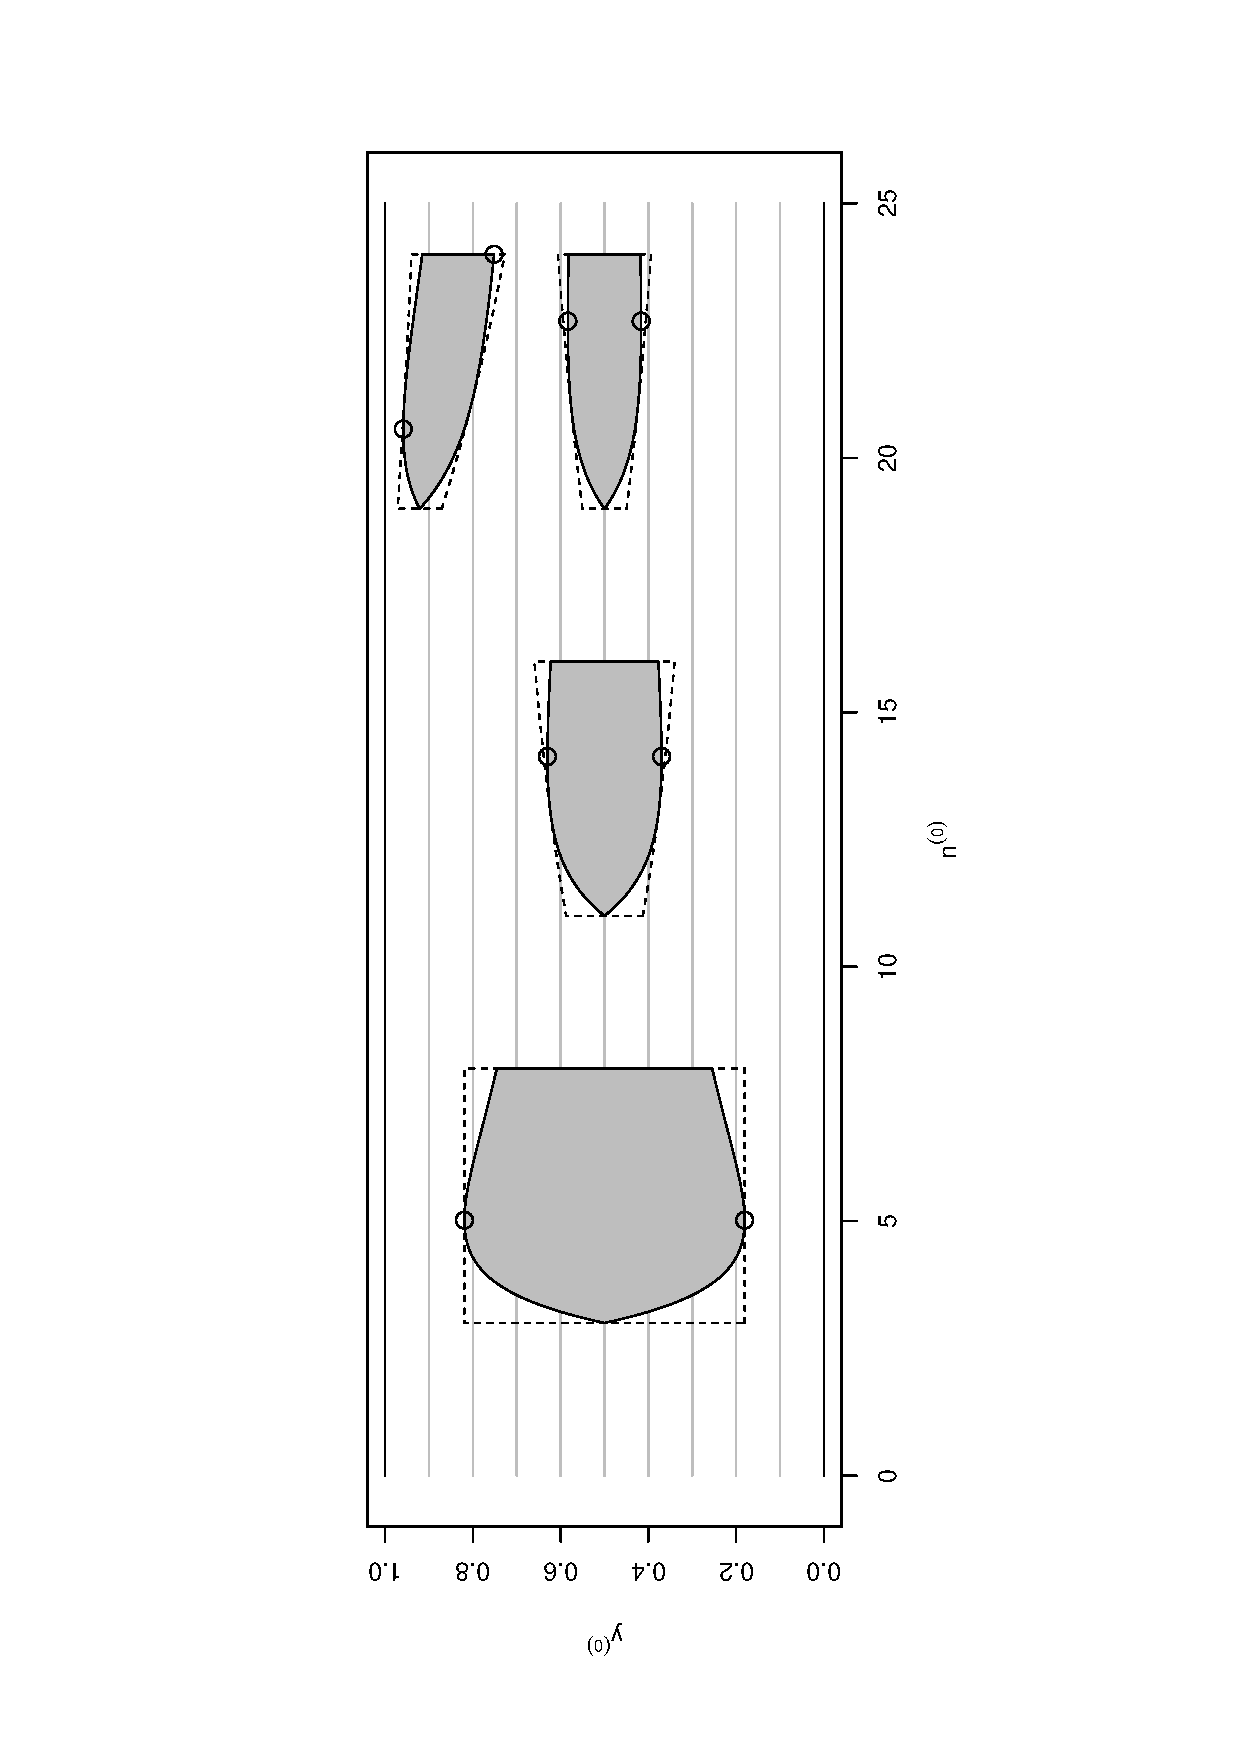
\includegraphics[trim = 40mm 35mm 40mm 45mm, clip, width=\textwidth]{../R/boatshape-durham0913} % width=8, height=6
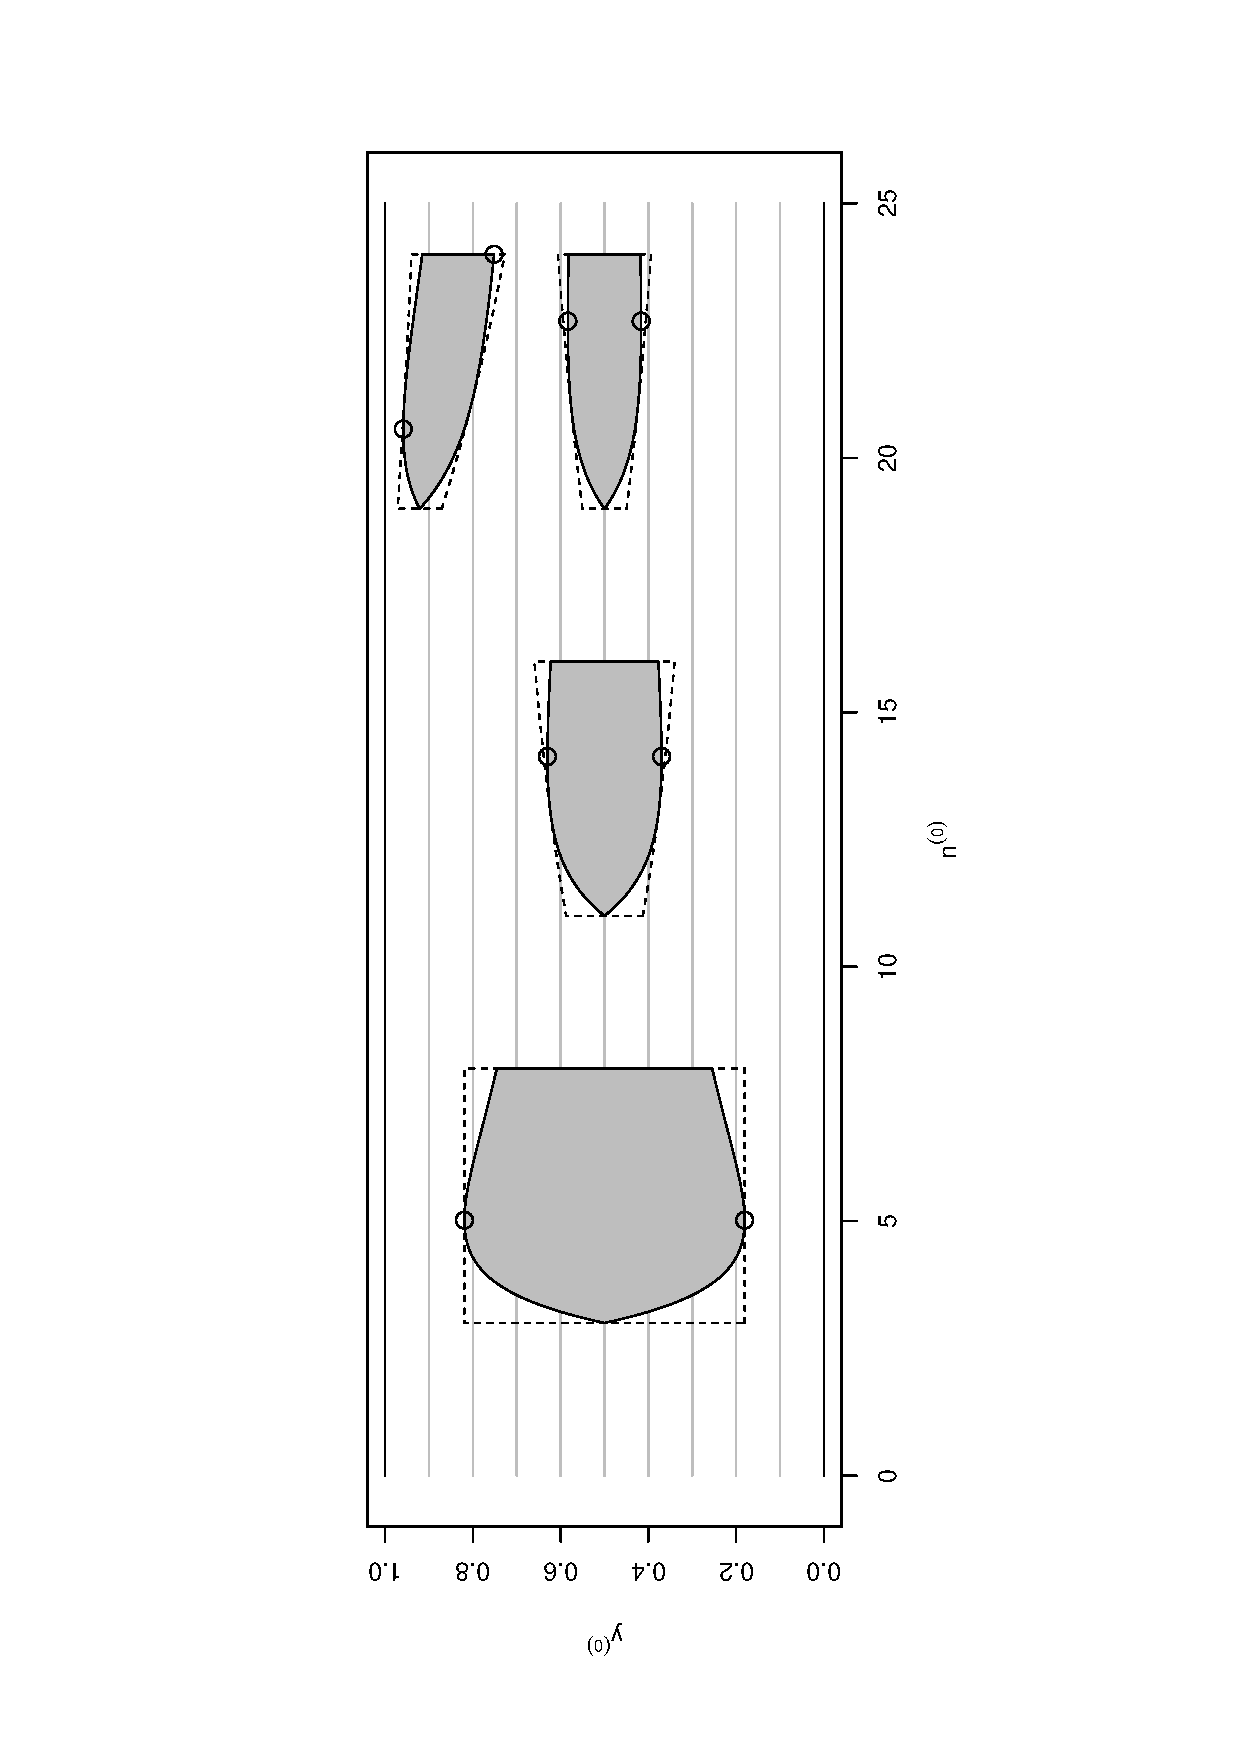
\includegraphics[trim = 70mm 52.5mm 70mm 65mm, clip, width=\textwidth]{../R/boatshape-durham0913} % width=6, height=4.5
\end{center}%}

}


\section{Common-Cause Failure Modeling}

\subsection{Common-Cause Failures}

\frame{\frametitle{Common-Cause Failures}
\begin{tikzpicture}
\uncover<1->{
\node {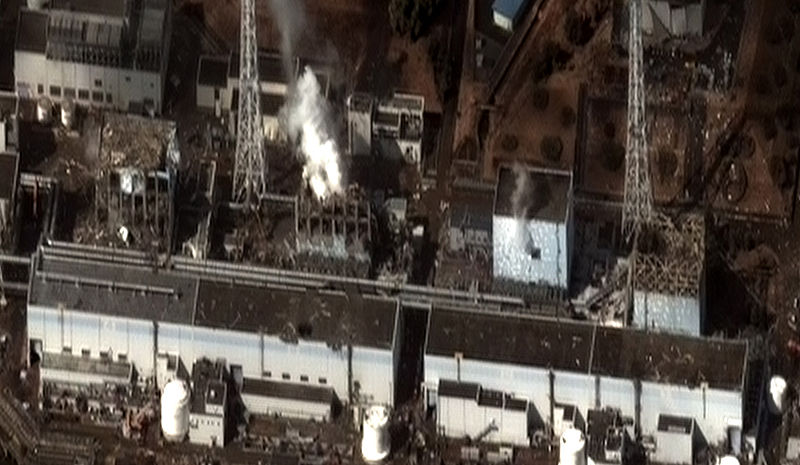
\includegraphics[scale=0.4]{./graph/800px-Fukushima_I_by_Digital_Globe.jpg}};
\node at (0,-3.5) {\tiny Source: Wikimedia Commons, \url{http://commons.wikimedia.org/wiki/File:Fukushima_I_by_Digital_Globe.jpg}};
}
\uncover<2->{
%\draw[white,fill=white] (-5,1) rectangle (5,3);
\node at (0,2.6) {\parbox{\textwidth}{
 \begin{alertblock}{common-cause failure} 
 \emph{simultaneous failure of several redundant components\\ due to a common or shared root cause}
 (H{\o}yland \& Rausand, 1994)
 \end{alertblock}
}};
}
\uncover<3>{
\draw[white,fill=white] (-0.2,-3.3) rectangle (6,0.75);
\node at (3,-1) {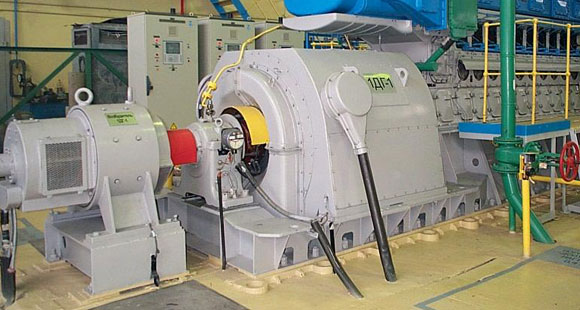
\includegraphics[scale=0.3]{./graph/plant-systems-diesel-generator.jpg}};
\node at (3.05,-3.05) {\parbox{6.2cm}{\tiny Source: \url{http://www.diakont.com/solutions/nuclear-energy/plant-systems/diesel-generator-control-systems/}}};
}
\end{tikzpicture}
}

\frame{\frametitle{Common-Cause Failure Modeling}


\begin{itemize}[<+->]
\item Crucial for overall system reliability analysis
\item \alert{Alpha factor model} is based on the Dirichlet-Multinomial model:\\
{\small categories $1,2,3,\ldots = 1,2,3,\ldots$ components failing simultaneously}
\item Informative Dirichlet priors elicited from experts\\ as data are sparse (zero counts for multi-component failures)
\item Non-informative priors are unsatisfactory:
 \begin{itemize}
 \item posterior is very sensitive to choice of prior
 \item which non-informative prior should we adopt?
 \end{itemize}
\item Troffaes, Walter \& Kelly (2013): sets of Dirichlet priors %(IDM, Walley 1996)
%\item Prior-data conflict sensitivity especially important for multi-component failures
\item More cautious inferences if prior and data are in conflict\\
(especially important for multi-component failures!)
\item Simple ways to elicit bounds for hyperparameters\\ by reasoning on hypothetical data
\end{itemize}

}

\subsection{Conclusion}

\frame{\frametitle{Conclusion}

\begin{itemize}%[<+->]
\item<1-> Conjugate priors are a convenient tool for Bayesian inference\\ but there are some pitfalls
 \begin{itemize}%[<+->]
 \item Hyperparameters $\nzg,\yzr$ are easy to interpret and elicit
 \item Averaging property makes calculations simple, but leads to
 inadequate model behaviour in case of \pdc
 \end{itemize}
\item<2-> Sets of conjugate priors maintain advantages \& mitigate issues %find a sweet spot in between
 \begin{itemize}%[<+->]
 \item Hyperparameter set shape is important %a crucial modeling choice
 \item Reasonable choice: \emph{rectangular} $\PZc = [\nzlg, \nzug] \times [\yzlr, \yzur]$
 \item Bounds for hyperparameters easy to interpret and elicit
 \item Additional imprecison in case of \pdc\\
 leads to \alert{cautious inferences if, and only if, caution is needed}
 \item Shape for more precision in case of strong prior-data agreement is in development
 (joint work with Frank Coolen and Mi\c{k} Bickis)
 \end{itemize}
\end{itemize}

}


\frame{\frametitle{References}

\nocite{2006:evans,1996:walley::idm,1991:walley,2005:quaeghebeurcooman-short,
Walter2009a-short,luck-package,Troffaes2013a,1994:hoyland,2012:benavolizaffalon-short}
%1965:good,2011:kelly:atwood,1996:atwood,}

\printbibliography[heading=none]

%\bibliographystyle{plainnat}
%\bibliography{../bib/eigene,../bib/itip-refs,../bib/other-refs}
}

\end{document}
